%!TEX root = ../operads_paper.tex
\section{Introduction}
QQQ Needs an intro. Might be something salvageable from the original papers.

Original paper intro:

Operads were defined by May \cite{maygeom} in the early 70's to provide a convenient tool to approach problems in algebraic topology, notably the question of when a space $X$ admits an $n$-fold delooping $Y$ so that $X \simeq \Omega^{n}Y$.  An operad, like an algebraic theory \cite{lawvere-thesis}, is something like a presentation for a monad or algebraic structure.  The theory of operads has seen great success, and we would like to highlight two reasons.  First, operads can be defined in any suitable symmetric monoidal category, so that there are operads of topological spaces, of chain complexes, of simplicial sets, and of categories, to name a few examples.  Moreover, symmetric (lax) monoidal functors carry operads to operads, so we can use operads in one category to understand objects in another via transport by such a functor.  Second, operads in a fixed category are highly flexible tools.  In particular, the categories listed above all have some inherent notion of ``homotopy equivalence'' which is weaker than that of isomorphism, so we can study operads which are equivalent but not isomorphic.  These tend to have algebras which have similar features in an ``up-to-homotopy'' sense but very different combinatorial or geometric properties arising from the fact that different objects make up these equivalent but not isomorphic operads.

Operads in the category $\mb{Cat}$ of small categories have a unique flavor arising from the fact that $\mb{Cat}$ is not just a category but a 2-category.  These 2-categorical aspects have not been widely treated in the literature, although a few examples can be found.  Lack \cite{lack-cod} mentions braided $\mb{Cat}$-operads (the reader new to braided operads should refer to the work of Fiedorowicz \cite{fie-br}) in his work on coherence for 2-monads, and Batanin \cite{bat-eh} uses lax morphisms of operads in $\mb{Cat}$ in order to define the notion of an internal operad.  But aside from a few appearances, the basic theory of operads in $\mb{Cat}$ and their 2-categorical properties seems missing.  This paper was partly motivated by the need for such a theory to be explained from the ground up.

There were two additional motivations for the work in this paper.  In thinking about coherence for monoidal functors, the first author was led to a general study of algebras for multicategories internal to $\mb{Cat}$.  These give rise to 2-monads (or perhaps pseudomonads, depending on how the theory is set up), and checking abstract properties of these 2-monads prompts one to consider the simpler case of operads in $\mb{Cat}$ instead of multicategories.  The other motivation was from the second author's attempt to understand the interplay between operads in $\mb{Cat}$, operads in $\mb{Top}$, and the passage from (bi)permutative categories to $E_{\infty}$ (ring) spaces.  The first of these motivations raised the issue of when operads in $\mb{Cat}$ are cartesian, while the second led us to consider when an operad in $\mb{Cat}$ possesses a pseudo-commutative structure.

While considering how to best tackle a general discussion of operads in $\mb{Cat}$, it became clear that restricting attention to the two most commonly used types of operads, symmetric and non-symmetric operads, was both short-sighted and unnecessary.  Many theorems apply to both kinds of operads at once, with the difference in proofs being negligible; in fact, most of the arguments which applied to the symmetric case seemed to apply to the case of braided operads as well.   This led us to the notion of an action operad $\mb{G}$, and then to a definition of $\mb{G}$-operads.  In essence, this is merely the general notion of what it means for an operad $P = \{ P(n) \}_{n \in \N}$ to have groups of equivariance $\mb{G} = \{ G(n) \}_{n \in \N}$ such that $G(n)$ acts on $P(n)$.  Choosing different natural families of groups $\mb{G}$, we recover known variants of the definition of operad. \\ \begin{center}
\begin{tabular}{c|c}
Groups $\mb{G}$ & Type of operad  \\ \hline
Terminal groups & Non-symmetric operad \\
Symmetric groups & Symmetric operad \\
Braid groups & Braided operad \\
\end{tabular} \\ \end{center}
These definitions have appeared, with minor variations, in two sources of which we are aware.  In Wahl's thesis \cite{wahl-thesis}, the essential definitions appear but not in complete generality as she requires a surjectivity condition.  Zhang \cite{zhang-grp} also studies these notions\footnote{Zhang calls our action operad a \textit{group operad}.  We dislike this terminology as it seems to imply that we are dealing with an operad in the category of groups, which is not the case unless all of the maps $\pi_{n}:G(n) \rightarrow \Sigma_{n}$ are zero maps.}, once again in the context of homotopy theory, but requires the  superfluous condition that $e_{1} = \textrm{id}$ (see Lemma \ref{calclem}).

This paper consists of the following.  In Section 1, we give the definition of an action operad $\mb{G}$ and a $\mb{G}$-operad.  We develop this definition abstractly so as to apply it in any suitable symmetric monoidal category.   It is standard to express operads as monoids in a particular functor category using a composition tensor product.  In order to show that our $\mb{G}$-operads fit into this philosophy, we must work abstractly and use the calculus of coends together with the Day convolution product \cite{day-thesis}.  The reader uninterested in these details can happily skip them, although we find the route taken here to be quite satisfactory in justifying the axioms for an action operad $\mb{G}$ and the accompanying notion of $\mb{G}$-operad.  Many of our calculations are generalizations of those appearing in work of Kelly \cite{kelly-op}, although there are slight differences in flavor between the two treatments.
%Kelly:  On the operads of JP May

Section 2 works through the basic 2-categorical aspects of operads in $\mb{Cat}$.  We explain how every operad gives rise to a 2-monad, and show that all of the various 1-cells between algebras of the associated 2-monad correspond to the obvious sorts of 1-cells one might define between algebras over an operad in $\mb{Cat}$.  Similarly, we show that the algebra 2-cells, using the 2-monadic approach, correspond to the obvious notion of transformation one would define using the operad.

Section 3 studies three basic 2-categorical properties of an operad, namely the property of being finitary, the property of being 2-cartesian, and the coherence property.  The first of these always holds, as a simple calculation shows.  The second of these turns out to be equivalent to the action of $G(n)$ on $P(n)$ being free for all $n$, at least up to a certain kernel.  In particular, our characterization clearly shows that every non-symmetric operad is 2-cartesian, and that a symmetric operad is 2-cartesian if and only if the symmetric group actions are all free.  (It is useful to note that a 2-monad on $\mb{Cat}$ is 2-cartesian if and only if the underlying monad on the category of small categories is cartesian in the usual sense as the (strict) 2-pullback of a diagram is the same as its pullback.)  The third property is also easily shown to hold for any $\mb{G}$-operad on $\mb{Cat}$ using a factorization system argument due to Power \cite{power-gen}.

Section 4 then goes on to study the question of when a $\mb{G}$-operad $P$ admits a pseudo-commutative structure.  Such a structure provides the 2-category of algebras with a richer structure that includes well-behaved notions of tensor product, internal hom, and multilinear map that fit together much as the analogous notions do in the category of vector spaces.  When $P$ is contractible (i.e., each $P(n)$ is equivalent to the terminal category), this structure can be obtained from a collection of elements $t_{m,n} \in G(mn)$ satisfying certain properties.  In particular, we show that every contractible symmetric operad is pseudo-commutative, and we prove that there exist such elements $t_{m,n} \in Br_{mn}$ so that every contractible braided operad is pseudo-commutative as well (in fact in two canonical ways).  Thus Section 4 can be seen as a continuation, in the operadic context, of the work in \cite{HP}, and in particular the ``geometric'' proof of the existence of a pseudo-commutative structure for braided strict monoidal categories demonstrates the power of being able to change the groups of equivariance.

The authors would like to thank John Bourke, Martin Hyland, Tom Leinster, and Peter May for various conversations which led to this paper.  While conducting this research, the second author was supported by an EPSRC Early Career Fellowship. 

Original Borel intro:


Categories of interest are often monoidal: sets, topological spaces, and vector spaces are all symmetric monoidal, while the category of finite ordinals (under ordinal sum) is merely monoidal.  But other categories have more exotic monoidal structures.  The first such type of structure discovered was that of a braided monoidal category.  These arise in categories whose morphisms have a geometric flavor like cobordisms embedded in some ambient space \cite{js}, in  categories produced from double loop spaces \cite{fie-br}, and categories of representations over objects like quasitriangular (or braided) bialgebras \cite{street-quantum} .  Another such exotic monoidal structure is that of a coboundary category, arising in examples from the representation theory of quantum groups \cite{drin-quasihopf}.

Going back to the original work of May on iterated loop spaces \cite{maygeom}, operads were defined in both symmetric and nonsymmetric varieties.  But Fiedorowicz's work on double loop spaces \cite{fie-br} showed that there was utility in considering another kind of operad, this time with braid group actions instead of symmetric group actions.  There is a clear parallel between these definitions of different types of operads and the definitions of different kinds of monoidal category, with each given by some general schema in which varying an $\mathbb{N}$-indexed collection of groups produced the types of operads or monoidal categories seen in nature.  Building on the work in \cite{cg}, the goal of this paper is to show that this parallel can be upgraded from an intuition to precise mathematics using the notion of action operad.

An action operad $\mb{\Lambda}$ is an operad which incorporates all of the essential features of the operad of symmetric groups.  Thus $\Lambda(n)$ is no longer just a set, but instead also has a group structure together with a map $\pi_{n}:\Lambda(n) \to \Sigma_{n}$.  Operadic composition then satisfies an additional equivariance condition using the maps $\pi_n$ and the group structures.  Each action operad $\mb{\Lambda}$ produces a notion of $\mb{\Lambda}$-operad which encodes equivariance conditions using both the groups $\Lambda(n)$ and the maps $\pi_n$.  Examples include the symmetric groups, the terminal groups (giving nonsymmetric operads), the braid groups (giving braided operads), and the $n$-fruit cactus groups \cite{hk-cobound} (giving a new notion of operad one might call cactus operads).  Using a formula resembling the classical Borel construction for spaces with a group action, we can produce from any action operad $\mb{\Lambda}$ a notion of $\mb{\Lambda}$-monoidal category, in which the group $\Lambda(n)$ acts naturally on $n$-fold tensor powers of any object.  Thus the categorical Borel construction embeds action operads into a category of monads on $\mb{Cat}$, and we characterize the image of this embedding as those monads describing monoidal structures of a precise kind.

The paper is organized into the following sections.  Section 1 reviews the definition of an action operad, and defines the categorical Borel construction on them.  The key result, which reappears in proofs throughout the paper, is \cref{thm:charAOp}, characterizing action operads in terms of two new operations mimicking the block sum of permutations and the operation which takes a permutation of $n$ letters and produces a new permutation on $k_1 + k_2 + \cdots + k_n$ letters by permuting the blocks of $k_i$ letters.  In Section 2, we use this characterization and Kelly's theory of clubs \cite{kelly_club1, kelly_club0, kelly_club2} to embed action operads into monads on $\mb{Cat}$ and determine the essential image of this embedding.  Section 3 gives a construction of the free action operad from a suitable collection of data, and relates this to how clubs can be described using generators and relations.  The results of Sections 2 and 3 show that the definitions of symmetric monoidal category or coboundary category, for example, correspond to the action operad constructed from the corresponding free symmetric monoidal or coboundary category on one object; these and other examples appear in detail in Section 4.  Section 5 then extends the definition of $\mb{\Lambda}$-operad to that of $\mb{\Lambda}$-multicategory and shows that these arise abstractly via a Kleisli construction.

Copied from text:
Yau \cite{yau_infinity_2021} collects together a large number of results on the topic of action operads while also investigating the setting of infinity group operads. 

This research was supported by EPSRC 134023.

Further acknowledgements:
Alex needs to thank the LMS for a Research Reboot grant. Anybody else we've talked to about these things since their inception? Angelica? Niles? Dan Graves. Nathaniel Arkor.




\section{Notation and Conventions}\label{sec:notation}

\begin{nota}[(Symmetric groups)]\label{nota:symm_sigma}
We denote the symmetric group on the symbols $1, 2, \ldots, n$ by $\Sigma_n$. Elements of a symmetric group are usually denoted by lowercase Greek letters or written in cycle notation.
\end{nota}

\begin{nota}[(Braid groups)]\label{nota:braid}
We denote the braid group on $n$ strands by $B_n$.
\end{nota}

\begin{nota}[(Identity elements)]\label{nota:e_identity}
The symbol $e$ will generically represent an identity element in a group. If we are considering a set of groups $\{ \Lambda(n) \}_{n \in \N}$ indexed by the natural numbers, then $e_{n}$ is the identity element in $\Lambda(n)$. We will often drop the subscripts and just write $e$ when the index $n$ in $\Lambda(n)$ is either clear from context or unimportant to the argument at hand.
\end{nota}

\begin{conv}[(Identity morphisms)]\label{conv:1_id}
We generically write an identity morphism $A \to A$ as either $1$ or $1_A$.
\end{conv}

\begin{nota}[(Group actions)]\label{nota:g-action}
For a group $G$, a right $G$-action on a set $X$ will be denoted $(x,g) \mapsto x \cdot g$ or $(x,g) \mapsto x g$. 
Similar notation will be used for left actions, and for multiplication in a group.
\end{nota}

\begin{conv}[(Indexed objects)]\label{conv:indexed}
We generically write $\{ \Lambda(n) \}_{n \in \N}$ for a $\N$-indexed family of objects $\Lambda(n)$. We will occasionallywrite $\Lambda_n$ in place of $\Lambda(n)$, especially in diagrams or when the objects $\Lambda_n$ have been independently defined, as in \cref{nota:symm_sigma,nota:braid}.
\end{conv}

\begin{conv}[(Products and quotients)]\label{conv:coeq}
We will often be interested in elements of a product of the form
\[
A \times B(1) \times \cdots \times B(n) \times C
\]
(or similar, for example without $C$). We will write elements of this set as $(a; b_{1}, \ldots, b_{n}; c)$, where $b_i \in B(i)$. 
In the case that we need to consider equivalence classes of such elements, these classes will be written as $[a; b_{1}, \ldots, b_{n}; c]$. 
The most common situation in which we consider such equivalence classes is that of a coequalizer of left and right group actions in the following sense. 
A coequalizer of maps
    \[
        \xy
            (0,0)*+{A \times G \times B}="00";
            (30,0)*+{A \times B}="10";
            (60,0)*+{\coeqb{A}{B}{G}}="20";
            {\ar@<1ex>^{1 \times \lambda} "00" ; "10"};
            {\ar@<-1ex>_{\rho \times 1} "00" ; "10"};
            {\ar^{\varepsilon} "10" ; "20"};
        \endxy
    \]
will be written as $\coeqb{A}{B}{G}$, where $\rho$ is a right action of $G$ on $A$ and $\lambda$ is a left action of $G$ on $B$. 
This notation is meant to emphasize the analogy with tensor products of $R$-modules, even when the monoidal structure involved is cartesian.
It also differentiates these coequalizers from pullbacks.
\end{conv}


\begin{conv}[(Pullbacks)]\label{conv:pb}
The pullback of the diagram
    \[
        \xy
            (10,0)*+{X}="00";
            (0,-10)*+{Y}="10";
            (10,-10)*+{A}="20";
            {\ar^{f} "00" ; "20"};
            {\ar_{g} "10" ; "20"};
        \endxy
    \]
will be written as $X \times_A Y$. 
\end{conv}

\begin{Defi}](Underlying permutation)]\label{Defi:underlying-perm}
Suppose that $f \colon G \to \Sigma_n$ is a given group homomorphism, and $x \in G$. The \emph{underlying permutation} of $x$ is the element $f(x) \in \Sigma_n$. If there is likely to be some confusion as to which homomorphism $f$ is being used, we will call $f(x)$ the \emph{underlying permutation with respect to $f$}.
\end{Defi}

\begin{nota}[(Applying underlying permutations)]\label{nota:perm_shorthand}
Throughout we will be using maps $\pi_n \colon O(n) \rightarrow \Sigma_n$, where $O(n)$ is the set of $n$-ary operations of an operad $O$ and $\Sigma_n$ is the symmetric group on $n$ elements.  
For any $\sigma \in O(n)$, we will write $\sigma(i)$ for $\pi_n(\sigma)(i)$, the image of $i$ with respect to the underlying permutation of $\sigma$; the notation $\sigma^{-1}(i)$ will be used for the inverse image of $i$ with respect to the underlying permutation of $\sigma$.
\end{nota}



\begin{Defi}[(Block sum)]\label{Defi:beta-s}
Let $k_1, \ldots, k_n$ be natural numbers and suppose that $\sigma_i \in \Sigma_{k_i}$ are permutations. The \emph{block sum} of $\sigma_1, \ldots, \sigma_n$, written 
\[
\beta( \sigma_1, \ldots, \sigma_n ),
\]
is the permutation in $\Sigma_K$, where $K = \sum_{i=1}^n k_i$, given as described below. 
For $1 \leq j \leq K$, define $c$ to be the unique integer such that
\[
k_1 + \cdots + k_c < j \leq k_1 + \cdots + k_c +k_{c+1}.
\]
Define
\[
\beta( \sigma_1, \ldots, \sigma_n )(j) = k_1 + \cdots + k_c + \sigma_{c+1}\big( j - (\sum_{i=1}^c k_i) \big).
\]
\end{Defi}

\begin{rem}\label{rem:beta-s}
The formula above expresses the idea that $\beta( \sigma_1, \ldots, \sigma_n )$ permutes the first $k_1$ elements using $\sigma_1$, the next $k_2$ elements using $\sigma_2$, and so on.
\end{rem}

\begin{Defi}[(Duplication)]\label{Defi:delta-s}
Let $k_1, \ldots, k_n$ be natural numbers, and suppose that $\sigma \in \Sigma_n$ is a permutation. The \emph{duplication} of $\sigma$ with respect to $k_1, \ldots, k_n$, written
\[
\delta_{n; k_1, \ldots, k_n}(\sigma),
\]
is the permutation in $\Sigma_K$, where $K = \sum_{i=1}^n k_i$, given as described below. 
For $1 \leq j \leq K$, define $c$ to be the unique integer such that
\[
k_1 + \cdots + k_c < j \leq k_1 + \cdots + k_c +k_{c+1}.
\]
Define
\[
\delta_{n; k_1, \ldots, k_n}(\sigma)(j) = \big( \sum_{\sigma(k_i) < \sigma(k_{c+1})} k_i\big) + j - \big( \sum_{i=1}^c k_i \big).
\]
\end{Defi}

\begin{rem}\label{rem:delta-s}
The formula above for $\delta_{n; k_1, \ldots, k_n}(\sigma)$ is best explained by drawing the graph of $\sigma$ as follows. The function $\sigma$ can be represented by drawing two rows of $n$ dots each, and connecting dot $i$ in the top row to dot $\sigma(i)$ in the bottom row. Then $\delta_{n; k_1, \ldots, k_n}(\sigma)$ is obtained by 
\begin{itemize}
\item replacing dot $i$ in the top row with $k_i$ dots,
\item replacing dot $\sigma(i)$ in the bottom row with $k_i$ dots, and
\item connecting these two sets of $k_i$ dots in the unique way that preserves order.
\end{itemize}
Thus we see that the $i$th entry for $\sigma$ is duplicated $k_i$ times in $\delta_{n; k_1, \ldots, k_n}(\sigma)$.
\end{rem}

\begin{rem}\label{rem:forward-matrices}
Figure out where to put these matrices in
\cref{rem:perm_matrices}.
\end{rem}

\begin{conv}[(Superscripts)]\label{conv:superscripts}
We generically use superscripts, when needed, to distinguish between operations of the same type associated to different structures. As an example, a monoid homomorphism $f \colon A \to B$ would have axioms written as
\begin{align*}
f(x \cdot^A y) & = f(x) \cdot^B f(y), \\
f(1^A) & = 1^B.
\end{align*}
\end{conv}

%\begin{conv}\label{conv1}
%We adopt the following conventions throughout.
%\begin{enumerate}
%\item\label{conv:symm_sigma} $\Sigma_{n}$ is the symmetric group on $n$ letters, and $B_{n}$ is the braid group on $n$ strands.
%\item\label{conv:g-action} For a group $G$, a right $G$-action on a set $X$ will be denoted $(x,g) \mapsto x \cdot g$. We will use both $\cdot$ and concatenation to represent multiplication in a group.
%\item\label{conv:e_identity} The symbol $e$ will generically represent an identity element in a group. If we are considering a set of groups $\{ \Lambda(n) \}_{n \in \N}$ indexed by the natural numbers, then $e_{n}$ is the identity element in $\Lambda(n)$. We will often drop the subscripts and just write $e$ when the index $n$ in $\Lambda(n)$ is either clear from context or unimportant to the argument at hand. Occasionally we will write $\Lambda_n$ in place of $\Lambda(n)$, especially in diagrams.
%\item\label{conv:coeq} We will often be interested in elements of a product of the form
%\[
%A \times B_{1} \times \cdots \times B_{n} \times C
%\]
%(or similar, for example without $C$). We will write elements of this set as $(a; b_{1}, \ldots, b_{n}; c)$, and in the case that we need equivalence classes of such elements they will be written as $[a; b_{1}, \ldots, b_{n}; c]$. This will often be the case when we are interested in the coequalizer of left and right group actions in the following sense. A coequalizer of maps
%    \[
%        \xy
%            (0,0)*+{A \times G \times B}="00";
%            (30,0)*+{A \times B}="10";
%            (60,0)*+{\coeqb{A}{B}{G}}="20";
%            {\ar@<1ex>^{\lambda} "00" ; "10"};
%            {\ar@<-1ex>_{\rho} "00" ; "10"};
%            {\ar^{\varepsilon} "10" ; "20"};
%        \endxy
%    \]
%will be written as $\coeqb{A}{B}{G}$, where $\rho$ represents a right action of $G$ on $A$, and $\lambda$ a left action of $G$ on $B$. This is similar to the notation often used to denote pullbacks, however we find in this work that no confusion arises from using notation in this way.
%\item\label{conv:beta_delta} In the following definitions of operads, we define operad multiplication as a function
%  \[
%    \mu \colon O(n) \times O(k_1) \times \ldots O(k_n) \rightarrow O(k_1 + \ldots + k_n)
%  \]
%for each $n$, $k_1$, $\ldots$, $k_n$, and we use the following two functions as a shorthand for two commonly occuring instances of such. First we define a function
%  \[
%    \beta \colon O(k_1) \times \ldots \times O(k_n) \rightarrow O(k_1 + \ldots + k_n)
%  \]
%for each $n$, $k_1$, $\ldots$, $k_n$, which takes elements $\tau_1 \in O(k_1)$, $\ldots$, $\tau_n \in O(k_n)$ and produces the element
%  \[
%    \beta(\tau_1, \ldots, \tau_n) = \mu(e_n; \tau_1, \ldots, \tau_n).
%  \]
%We think of this element as the block sum of the elements $\tau_1$, $\ldots$, $\tau_n$. We also define a function
%  \[
%    \delta_{n;k_1,\ldots,k_n} \colon O(n) \rightarrow O(k_1 + \ldots + k_n)
%  \]
%for each $n$, $k_1$, $\ldots$, $k_n$, which takes an element $\sigma \in O(n)$ and produces the element
%  \[
%    \delta(\sigma) = \mu(\sigma;e_{k_1}, \ldots, e_{k_n}).
%  \]
%
%In the particular case of the symmetric groups, these are functions
%  \[
%    \beta \colon \Sigma_{k_1} \times \Sigma_{k_n} \rightarrow \Sigma_{k_1 + \ldots + k_n}
%  \]
%and
%  \[
%    \delta_{n;k_1,\ldots,k_n} \colon \Sigma_{n} \rightarrow \Sigma_{k_1 + \ldots + k_n}.
%  \]
%In the case of $\beta$ we form the block sum permutation $\beta(\tau_1,\ldots,\tau_n)$ which permutes the first $k_{1}$ elements according to $\tau_{1}$, the next $k_{2}$ elements according to $\tau_{2}$ and so on; this is an element of $\Sigma_{k_{1} + \cdots + k_{n}}$. For $\delta$ we take the permutation $\delta(\sigma) \in \Sigma_{k_{1} + \cdots + k_{n}}$ to be that which permutes the $n$ different blocks $1$ through $k_{1}$, $k_{1}+1$ through $k_{1} + k_{2}$, and so on, according to the permutation $\sigma \in \Sigma_{n}$. We expand on this at various points, including in \cref{rem:perm_matrices}.
%\item\label{conv:perm_shorthand} Throughout we will be using maps $\pi_n \colon O(n) \rightarrow \Sigma_n$, where $O(n)$ is the object of $n$-ary operations of an operad $O$ and $\Sigma_n$ is the symmetric group on $n$ elements. The map $\pi_n$ in each case will represent a form of `underlying permutation' of each element, which we will then use to act on operad multiplication. As the notation starts to become cumbersome, we will often write $\sigma^{-1}(i)$ which should be read as $\pi_n(\sigma)^{-1}(i)$, where $\sigma \in O(n)$.
%\item\label{conv:op_superscript} We adopt the convention that if an equation requires using operadic composition in more than one operad, we will indicate this by a superscript on each instance of $\mu$ unless it is entirely clear from context. This can be seen, for example, in \cref{Defi:op_map}.
%\end{enumerate}
%\end{conv}

\artpart{Operads and Action Operads}

\section{Background: Operads}\label{sec:back-op}

This section will collect the basic background information on operads that we will later generalize in\ngnote{ref later sections}. We begin with the most common type of operad, a symmetric operad, before defining two more types of operad: plain and braided. 

\begin{Defi}[(Symmetric operad)]\label{Defi:sym-op}
A \textit{symmetric operad} $O$ (in the category of sets) consists of
\begin{itemize}
\item a set, $O(n)$, for each natural number $n$,
\item for each $n$, a right $\Sigma_{n}$-action on $O(n)$,
\item an element $\id \in O(1)$, and
\item functions
  \[
    \mu \colon  O(n) \times O(k_{1}) \times \cdots \times O(k_{n}) \rightarrow O(k_{1} + \cdots + k_{n}),
  \]
\end{itemize}
satisfying the following three axioms.
\begin{enumerate}
\item The element $\id \in O(1)$ is a two-sided unit for $\mu$, meaning that
  \begin{align*}
    \mu(\id;x) &= x,\\
    \mu(x;\id,\ldots,\id) &= x
  \end{align*}
for any $x \in O(n)$.
\item The functions $\mu$ are associative, meaning that the diagram below commutes.
% \[
% \xy
% (0,0)*+{\scriptstyle O(n) \times O(k_{1}) \times \cdots \times O(k_{n}) \times O(l_{1,1}) \times \cdots \times O(l_{{1},k_{1}}) \times \cdots \times O(l_{n,1}) \times \cdots \times O(l_{{n},k_{n}})} ="00";
% (0,-50)*+{\scriptstyle O(k_{1} + \cdots + k_{n}) \times O(l_{1,1}) \times \cdots \times O(l_{{1},k_{1}}) \times \cdots \times O(l_{n,1})\times \cdots \times O(l_{{n},k_{n}})} ="02";
% (55,-10)*+{\scriptstyle O(n) \times \prod_{i=1}^n O(k_{i}) \times O(l_{i,1}) \times \cdots \times O(l_{{i}, k_{i}}) } ="20";
% (55,-25)*+{\scriptstyle O(n) \times O(\sum l_{1,-}) \times \cdots \times O(\sum l_{n,-})} ="21";
% (55, -40)*+{\scriptstyle  O(\sum l_{-,-})} ="22";
% {\ar_{\scriptstyle \mu \times 1} "00" ; "02"};
% {\ar_{\mu} "02" ; "22"};
% {\ar^{\cong} "00" ; "20"};
% {\ar^{1 \times \prod \mu} "20" ; "21"};
% {\ar^{\mu} "21" ; "22"};
% \endxy
% \]


  \[
    \xy
      (0,0)*+{\scriptstyle O(n) \times \left(\prod_{i=1}^n O(k_i)\right) \times \left(\prod_{i=1}^n\prod_{j=1}^{k_i} O(l_{i,j})\right)}="a";
      (65,0)*+{\scriptstyle O(n) \times \prod_{i=1}^n \left(O(k_i) \times \prod_{j=1}^{k_i} O(l_{i,j})\right)}="b";
      (65,-20)*+{\scriptstyle O(n) \times \prod_{i=1}^n O\left(\sum_{j=1}^{k_i} l_{i,j}\right)}="c";
      (65,-40)*+{\scriptstyle O\left(\sum_{i=1}^n \sum_{j=1}^{k_i} l_{i,j}\right)}="d";
      (0,-40)*+{\scriptstyle O\left(\sum_{i=1}^n k_i\right) \times \prod_{i=1}^n \prod_{j=1}^{k_i} O(l_{i,j})}="e";
      %
      {\ar^{\cong} "a" ; "b"};
      {\ar^{1 \times \prod \mu} "b" ; "c"};
      {\ar^{\mu} "c" ; "d"};
      {\ar_{\mu \times 1} "a" ; "e"};
      {\ar_{\mu} "e" ; "d"};
    \endxy
  \]

\item The functions $\mu$ are equivariant with respect to the symmetric group actions, meaning that two equations hold.
\begin{itemize}
\item[3.1] Suppose that $x \in O(n)$, $y_i \in O(k_i)$ for $i = 1, \ldots, n$, and $\tau_i \in \Sigma_{k_i}$ for  $i = 1, \ldots, n$. Then the first equivariance axiom is the requirement that
\[
\mu(x;y_1 \cdot \tau_1,\ldots,y_n \cdot \tau_n) = \mu(x;y_1,\ldots,y_n)\cdot \beta(\tau_1,\ldots,\tau_n)
\]
holds, where $\beta$ is the function from \cref{Defi:beta-s}.
\end{itemize}
\begin{itemize}
\item[3.2] Suppose that  $x \in O(n)$, $y_i \in O(k_i)$ for $i = 1, \ldots, n$, and $\sigma \in \Sigma_{n}$. 
Then the second equivariance axiom is the requirement that
\[
 \mu(x \cdot \sigma; y_1, \ldots, y_n) = \mu\left(x;y_{\sigma^{-1}(1)},\ldots,y_{\sigma^{-1}(n)}\right)\cdot \delta_{n; k_1, \ldots, k_n}(\sigma)
\]
holds, where $\delta_{n; k_1, \ldots, k_n}$ is the function from \cref{Defi:delta-s}.
\end{itemize}
%
%the following two equations hold.
%  \begin{align*}
%    \mu(x;y_1 \cdot \tau_1,\ldots,y_n \cdot \tau_n) &= \mu(x;y_1,\ldots,y_n)\cdot \beta(\tau_1,\ldots,\tau_n)\\
%    \mu(x \cdot \sigma; y_1, \ldots, y_n) &= \mu\left(x;y_{\sigma^{-1}(1)},\ldots,y_{\sigma^{-1}(n)}\right)\cdot \delta(\sigma)
%  \end{align*}
%  % \begin{align*}
%  %   \mu(x;y_1 \cdot \tau_1,\ldots,y_n \cdot \tau_n) &= \mu(x;y_1,\ldots,y_n)\cdot(\tau_1 \oplus \ldots \oplus \tau_n)\\
%  %   \mu(x \cdot \sigma; y_1, \ldots, y_n) &= \mu\left(x;y_{\sigma^{-1}(1)},\ldots,y_{\sigma_{-1}(n)}\right)\cdot \sigma^+
%  % \end{align*}
%  For the first equation above, we 
\end{enumerate}
\end{Defi}

\begin{term}[(Operadic multiplication, composition)]\label{term:operadic-mult}
The functions $\mu$ in \cref{Defi:sym-op} are called \emph{operadic multiplication} or \emph{operadic composition} maps.
\end{term}

\begin{rem}\label{rem:op-def}
One is intended to think that $x \in O(n)$ is a function with $n$ inputs and a single output, as below.
  \begin{center}
  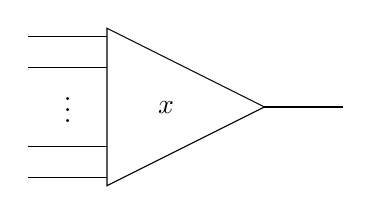
\begin{tikzpicture}
    \draw (0,0.9) -- (1,0.9);
    \draw (0,0.5) -- (1,0.5);
    %
    \node [anchor=center] () at (0.5,0) {$\vdots$\strut};
    %
    \draw (0,-0.5) -- (1,-0.5);
    \draw (0,-0.9) -- (1,-0.9);
    %
    \draw (1,1) -- (1,-1) -- (3,0) -- cycle;
    %
    \draw (3,0) -- (4,0);
    %
    \node [anchor=center] () at (1.75,0) {$x$\strut};
  \end{tikzpicture}
  \end{center}
  % \[
  %   \xy
  %     {\ar@{-} (0,0)*{}; (25,-10)*{} };
  %     {\ar@{-} (0,-20)*{}; (25,-10)*{} };
  %     {\ar@{-} (0,0)*{}; (0,-20)*{} };
  %     {\ar@{-} (25,-10)*{}; (35,-10)*{} };
  %     {\ar@{-} (0,0)*{}; (-10,0)*{} };
  %     {\ar@{-} (0,-3)*{}; (-10,-3)*{} };
  %     {\ar@{-} (0,-17)*{}; (-10,-17)*{} };
  %     {\ar@{-} (0,-20)*{}; (-10,-20)*{} };
  %     (11,-10)*{x}; (-5,-10)*{\vdots}
  %   \endxy
  % \]
Operadic composition is then a generalization of function composition, with the pictorial representation below being $\mu(x; y_{1}, y_{2})$ for $\mu \colon O(2) \times O(2) \times O(3) \rightarrow O(5)$.
  \begin{center}
  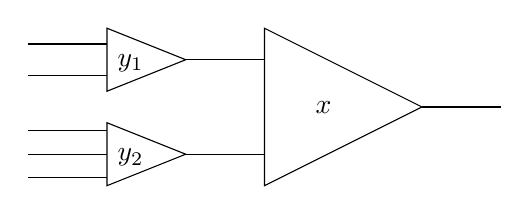
\begin{tikzpicture}
    % upper triangle
    \draw (-2,0.8) -- (-1,0.8);
    %
    \draw (-2,0.4) -- (-1,0.4);
    %
    \draw (-1,1) -- (-1,0.2) -- (0,0.6) -- cycle;
    %
    \node [anchor=center] () at (-0.7,0.6) {$y_1$\strut};    
    % lower triangle
    \draw (-2,-0.9) -- (-1,-0.9);
    %
    \draw (-2,-0.3) -- (-1,-0.3);
    %
    \draw (-1,-1) -- (-1,-0.2) -- (0,-0.6) -- cycle;
    %
    \draw (-2,-0.6) -- (-1,-0.6);
    %
    \node [anchor=center] () at (-0.7,-0.6) {$y_2$\strut};
    % big triangle
    \draw (0,0.6) -- (1,0.6);
    %    
    \draw (0,-0.6) -- (1,-0.6);
    %
    \draw (1,1) -- (1,-1) -- (3,0) -- cycle;
    %
    \draw (3,0) -- (4,0);
    %
    \node [anchor=center] () at (1.75,0) {$x$\strut};
  \end{tikzpicture}
  \end{center}
  % \[
  %   \xy
  %     {\ar@{-} (0,0)*{}; (25,-10)*{} };
  %     {\ar@{-} (0,-20)*{}; (25,-10)*{} };
  %     {\ar@{-} (0,0)*{}; (0,-20)*{} };
  %     {\ar@{-} (25,-10)*{}; (35,-10)*{} };
  %     {\ar@{-} (0,-3)*{}; (-10,-3)*{} };
  %     {\ar@{-} (0,-17)*{}; (-10,-17)*{} };
  %     (11,-10)*{x};
  %     {\ar@{-} (-25,2)*{}; (-10,-3)*{} };
  %     {\ar@{-} (-25,-8)*{}; (-10,-3)*{} };
  %     {\ar@{-} (-25,2)*{}; (-25,-8)*{} };
  %     {\ar@{-} (-25,1)*{}; (-30,1)*{} };
  %     {\ar@{-} (-30,-7)*{}; (-25,-7)*{} };
  %     (-19,-3)*{y_{1}};
  %     {\ar@{-} (-25,-12)*{}; (-10,-17)*{} };
  %     {\ar@{-} (-25,-22)*{}; (-10,-17)*{} };
  %     {\ar@{-} (-25,-12)*{}; (-25,-22)*{} };
  %     {\ar@{-} (-25,-13)*{}; (-30,-13)*{} };
  %     {\ar@{-} (-25,-17)*{}; (-30,-17)*{} };
  %     {\ar@{-} (-25,-21)*{}; (-30,-21)*{} };
  %     (-19,-17)*{y_{2}};
  %   \endxy
  % \]
  \end{rem}

\begin{term}[($n$-ary operations)]\label{term:nary-ops}
The set $O(n)$ in \cref{Defi:sym-op} is called the set of \emph{$n$-ary operations} of $O$.
\end{term}

\begin{rem}\label{rem:nary-ops-V}
If $O$ is an operad in a category other than $\mb{Sets}$ (see \cref{rem:V-and-coll}), then we would call $O(n)$ the \emph{object} of $n$-ary operations.
\end{rem}

%\begin{rem}\label{Rem:sigma_conditions}
%It is useful to write out in full what the sets in the diagram of the second axiom above mean. The use of numerous products and indices is to save space but the full picture becomes much clearer when these are expanded. For the equations in the third axiom above to make sense, we must have
%\begin{itemize}
%\item $x \in O(n)$,
%\item $y_{i} \in O(k_{i})$ for $i=1, \ldots, n$,
%\item $\tau_{i} \in \Sigma_{k_{i}}$,
%\item $\sigma \in \Sigma_{n}$, and
%\item $\beta(\tau_1,\ldots,\tau_n), \delta(\sigma) \in \Sigma_{k_1 + \ldots + k_n}$ as described in \cref{conv1} \eqref{conv:beta_delta}.
%\end{itemize}
%
%\end{rem}

Here are two important examples of symmetric operads.

\begin{example}[(Symmetric operad of symmetric groups)]\label{ex:Sigma}
The canonical example of \emph{a} symmetric operad is \emph{the} symmetric operad which we write as $\Sigma$. The set $\Sigma(n)$ is the set of elements of the symmetric group $\Sigma_{n}$, and the group action is just multiplication on the right. The identity element $\id \in \Sigma(1)$ is just the identity permutation on a one-element set. Operadic composition in $\Sigma$ will then be given by a function
  \[
    \Sigma(n) \times \Sigma(k_{1}) \times \cdots \times \Sigma(k_{n}) \rightarrow \Sigma(k_{1} + \cdots + k_{n})
  \]
which takes permutations $\sigma \in \Sigma_{n}, \tau_{i} \in \Sigma_{k_{i}}$ and produces the following permutation in $\Sigma_{k_{1} + \cdots + k_{n}}$:
  \[
    \mu(\sigma; \tau_{1}, \ldots, \tau_{n}) = \delta(\sigma) \cdot \beta(\tau_1,\ldots,\tau_n),
  \]
with $\beta$ and $\delta$ as in \cref{conv1}.

Below we have drawn the permutation for the composition
  \[
    \mu \colon \Sigma(3) \times \Sigma(2) \times \Sigma(4) \times \Sigma(3) \rightarrow \Sigma(9)
  \]
evaluated on the element $\left( (1 \,\, 2 \,\, 3); \trans{1}{2},\trans{1}{2}\trans{3}{4},\trans{1}{3} \right)$, in terms of $\beta$ and $\delta$. We expand on this in \cref{thm:charAOp}.
  \begin{center}
  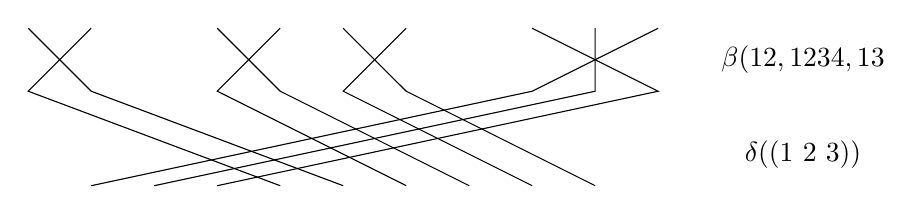
\begin{tikzpicture}[scale=0.8]
  \draw (1,0) -- (2,-1) -- (6,-2.5);
  \draw (2,0) -- (1,-1) -- (5,-2.5);
  \draw (4,0) -- (5,-1) -- (8,-2.5);
  \draw (5,0) -- (4,-1) -- (7,-2.5);
  \draw (6,0) -- (7,-1) -- (10,-2.5);
  \draw (7,0) -- (6,-1) -- (9,-2.5);
  \draw (9,0) -- (11,-1) -- (4,-2.5);
  \draw (10,0) -- (10,-1) -- (3,-2.5);
  \draw (11,0) -- (9,-1) -- (2,-2.5);
  \node at (13.3,-0.5) {$\beta(\trans{1}{2},\trans{1}{2}\trans{3}{4}, \trans{1}{3}$};
  \node at (13.3,-2) {$\delta((1 \,\, 2 \,\, 3))$};
  \end{tikzpicture}
  \end{center}
  % \[
  %   \xy
  %     {\ar@{-} (0,0)*{}; (5,-5)*{} };
  %     {\ar@{-} (5,0)*{}; (0,-5)*{} };
  %     {\ar@{-} (12,0)*{}; (17,-5)*{} };
  %     {\ar@{-} (17,0)*{}; (12,-5)*{} };
  %     {\ar@{-} (22,0)*{}; (27,-5)*{} };
  %     {\ar@{-} (27,0)*{}; (22,-5)*{} };
  %     {\ar@{-} (34,0)*{}; (44,-5)*{} };
  %     {\ar@{-} (39,0)*{}; (39,-5)*{} };
  %     {\ar@{-} (44,0)*{}; (34,-5)*{} };
  %     {\ar@{-} (0,-5)*{}; (17,-13)*{} };
  %     {\ar@{-} (5,-5)*{}; (22,-13)*{} };
  %     {\ar@{-} (12,-5)*{}; (29,-13)*{} };
  %     {\ar@{-} (17,-5)*{}; (34,-13)*{} };
  %     {\ar@{-} (22,-5)*{}; (39,-13)*{} };
  %     {\ar@{-} (27,-5)*{}; (44,-13)*{} };
  %     {\ar@{-} (34,-5)*{}; (0,-13)*{} };
  %     {\ar@{-} (39,-5)*{}; (5,-13)*{} };
  %     {\ar@{-} (44,-5)*{}; (10,-13)*{} };
  %   \endxy
  % \]
  
 \textbf{End this example here, with labels, move the rest to after 2.26.}

\begin{remark}\label{Rem:perm_matrices}
Permutations, as elements of $\Sigma_n$, can be considered as permutation \emph{matrices}, matrices with exactly one $1$ in each row and column. E.g., the permutation $(1 \,\, 3 \,\, 2) \in \Sigma_3$ can be considered as the matrix
  \[
  \begin{bmatrix}
  0 & 0 & 1 \\
  1 & 0 & 0 \\
  0 & 1 & 0
  \end{bmatrix},
  \]
which permutes three elements $  \begin{bmatrix} a & b & c \end{bmatrix}$ by pre-multiplying by the permutation matrix:
  \[
  \begin{bmatrix}
  0 & 0 & 1 \\
  1 & 0 & 0 \\
  0 & 1 & 0
  \end{bmatrix}
  \begin{bmatrix}
  a \\ b \\ c
  \end{bmatrix}
  =
  \begin{bmatrix}
  c \\ a \\ b
  \end{bmatrix}.
  \]
Then $\beta$ corresponds to the process of taking the block diagonal matrix of the original permutation matrices. So given elements $\trans{1}{2} \in \Sigma_2$, $e_1 \in \Sigma_1$, and $(1 \,\, 3 \,\, 2) \in \Sigma_3$, then
  \begin{align*}
  \beta(\trans{1}{2},e_1,(1 \,\, 2 \,\, 3)) &=
  \begin{bmatrix}
  \begin{bmatrix}
  0 & 1 \\
  1 & 0
  \end{bmatrix} & 0 & 0 \\
  0 & \begin{bmatrix} 1 \end{bmatrix} & 0 \\
  0 & 0 &   \begin{bmatrix}
  0 & 0 & 1 \\
  1 & 0 & 0 \\
  0 & 1 & 0
  \end{bmatrix}
  \end{bmatrix}\\
  &=
  \begin{bmatrix}
  0 & 1 & 0 & 0 & 0 & 0 \\
  1 & 0 & 0 & 0 & 0 & 0 \\
  0 & 0 & 1 & 0 & 0 & 0 \\
  0 & 0 & 0 & 0 & 0 & 1 \\
  0 & 0 & 0 & 1 & 0 & 0 \\
  0 & 0 & 0 & 0 & 1 & 0 \\
  \end{bmatrix} \\
  &= \trans{1}{2}(3)(4 \,\, 5 \,\, 6).
  \end{align*}
Similarly, we can describe $\delta$ as an operation on permutation matrices. The idea here is that for $\sigma \in \Sigma_n$, $\delta_{n;k_1,\ldots,k_n}(\sigma)$ takes a block diagonal of identity matrices $I_{k_1}$, $\ldots$, $I_{k_n}$ (which corresponds to $\beta(e_{k_1},\ldots,e_{k_n}) \in \Sigma_{k_1+\ldots+k_n}$), and permutes these according to the effect of the permutation $\sigma$. For example, given $\sigma = (1 \,\, 2 \,\, 3)$, then
  \[
    \delta_{3;2,1,3}(\sigma) =
    \begin{bmatrix}
    I_2 & 0 & 0 \\
    0 & I_1 & 0 \\
    0 & 0 & I_3
    \end{bmatrix}
    \ast
    \sigma
    =
      \begin{bmatrix}
      0 & 0 & 1 \\
      1 & 0 & 0 \\
      0 & 1 & 0
      \end{bmatrix}
    \ast
    \begin{bmatrix}
    I_2 & 0 & 0 \\
    0 & I_1 & 0 \\
    0 & 0 & I_3
    \end{bmatrix}
    =
    \begin{bmatrix}
    0 & 0 & I_3 \\
    I_2 & 0 & 0 \\
    0 & I_1 & 0
    \end{bmatrix}.
  \]
We make use of a similar interpretation of signed permutations and block diagonal matrices in a counterexample given in \cref{Ex:counterex}.
\end{remark}

  
Note that $(12)(34) \in \Sigma(4)$ is actually $\mu(e_{2}; (12), (12))$, where $e_{2} \in \Sigma_{2}$ is the identity permutation. Using this and operad associativity, one can easily check that
  \[
    \mu \left( (123); (12), (12)(34), (13) \right) = \mu \left( (1234); (12), (12), (12), (13) \right),
  \]
where now the composition on the right side uses the function
  \[
    \mu \colon \Sigma(4) \times \Sigma(2) \times \Sigma(2) \times \Sigma(2) \times \Sigma(3) \rightarrow \Sigma(9).
  \]
This equality is obvious using the picture above, but verifiable directly using only the algebra of the symmetric operad.
\end{example}

\begin{example}[(Endomorphism operad)]\label{ex:endo}
Let $X$ be a set. The \emph{endomorphism operad} of $X$, denoted $\mathcal{E}_X$, consists of 
\begin{itemize}
\item the sets
\[
\mathcal{E}_X(n) = \mb{Sets}(X^n, X),
\]
\item the right group actions $\mathcal{E}_X(n) \times \Sigma_n \to \mathcal{E}_X(n)$ given by
\[
(f \cdot \sigma)(x_1, \ldots, x_n) = f( x_{\sigma^{-1}(1)}, \ldots, x_{\sigma^{-1}(n)}),
\]
\item the element $\id \in \mathcal{E}_X(1)$ being the identity function $1 \colon X \to X$, and
\item operadic multiplication given by
\[
\mu(g; f_1, \ldots, f_n) = g \circ (f_1 \times \cdots \times f_n).
\]
\end{itemize}
We leave verification of the axioms to the reader, or recommend\ngnote{may-GoILS, find specific ref number}.
\end{example}

\begin{rem}
Intuition in \cref{rem:op-def} connected with example \cref{ex:endo} through the concept of an algebra, see\ngnote{later section} for these.
\end{rem}

One can also drop the symmetric group actions entirely to obtain the notion of a non-symmetric or plain operad.

\begin{Defi}[(Non-symmetric operad)]\label{Defi:non-sym-op}
A \emph{non-symmetric operad} $O$ consists of 
\begin{itemize}
\item a set, $O(n)$, for each natural number $n$,
%\item for each $n$, a right $\Sigma_{n}$-action on $O(n)$,
\item an element $\id \in O(1)$, and
\item functions
  \[
    \mu \colon  O(n) \times O(k_{1}) \times \cdots \times O(k_{n}) \rightarrow O(k_{1} + \cdots + k_{n}),
  \]
\end{itemize}
satisfying axioms 1 and 2 from \cref{Defi:sym-op}.
\end{Defi}

\begin{rem}\label{rem:V-and-coll}
\begin{enumerate}
\item One can change from operads in $\mb{Sets}$ to operads in another (symmetric) monoidal category $\mathcal{V}$ by requiring each $O(n)$ to be an object of $\mathcal{V}$ and replacing all instances of cartesian product with the appropriate tensor product in $\mathcal{V}$. One would also the element $\id \in O(1)$ with a map $I \rightarrow O(1)$ from the unit object of $\mathcal{V}$ to $O(1)$. In the case of symmetric operads, one would also express the right group actions as homomorphisms
\[
\Sigma_n^{op} \to \mathcal{V}\big( O(n), O(n) \big).
\]
\item Every symmetric operad has an underlying \textit{symmetric collection} which consists of the natural number-indexed set $\{ O(n) \}_{n \in \N}$ together with symmetric group actions, but without a chosen identity element or composition maps. The category of symmetric collections is a presheaf category, and we will equip it with a monoidal structure in which monoids are precisely operads in \cref{operad=monoid}. A similar construction, but without reference to group actions, shows that every non-symmetric operad has an underlying (non-symmetric) collection which is now merely a $\N$-indexed collection of sets.
\end{enumerate}
\end{rem}

\begin{example}\label{ex:non-sym}
\ngnoteil{insert example of non-symmetric operad here, how about Trimble's thing in dimension 1?}
\end{example}

\cref{ex:non-sym}

In the original topological applications \cite{maygeom}, symmetric operads were the central figures. A further kind of operad was studied by Fiedorowicz in \cite{fie-br}, that of a \emph{braided} operad in which the braid groups take the place of the symmetric groups. We sketch that definition below, but postpone details to\ngnote{write this out later, ref back}.

\begin{Defi}[(Braided operad, sketch)]\label{Defi:broperad}
A \textit{braided operad} consists of
  \begin{itemize}
    \item a non-symmetric operad $O$ and
    \item for each $n$, a right action of the $n$th braid group $B_{n}$ on $O(n)$,
  \end{itemize}
%satisfying the following axioms.
%  \begin{align*}
%    \mu(x;y_1 \cdot \tau_1,\ldots,y_n \cdot \tau_n) &= \mu(x;y_1,\ldots,y_n)\cdot\beta(\tau_1,\ldots,\tau_n)\\
%    \mu(x \cdot \sigma; y_1, \ldots, y_n) &= \mu\left(x;y_{\sigma^{-1}(1)},\ldots,y_{\sigma^{-1}(n)}\right)\cdot \delta_{n; k_1, \ldots, k_n}(\sigma)
%  \end{align*}
%  
such that the operadic multiplication functions $\mu$ are equivariant with respect to the braid group actions, meaning that two equations hold.
\begin{itemize}
\item[1] Suppose that $x \in O(n)$, $y_i \in O(k_i)$ for $i = 1, \ldots, n$, and $\tau_i \in B_{k_i}$ for  $i = 1, \ldots, n$. Then the first equivariance axiom is the requirement that
\[
\mu(x;y_1 \cdot \tau_1,\ldots,y_n \cdot \tau_n) = \mu(x;y_1,\ldots,y_n)\cdot \beta(\tau_1,\ldots,\tau_n)
\]
holds.%, where $\beta$ is the function from \cref{Defi:beta-s}.
\item[2] Suppose that  $x \in O(n)$, $y_i \in O(k_i)$ for $i = 1, \ldots, n$, and $\sigma \in B_{n}$. 
Then the second equivariance axiom is the requirement that
\[
 \mu(x \cdot \sigma; y_1, \ldots, y_n) = \mu\left(x;y_{\sigma^{-1}(1)},\ldots,y_{\sigma^{-1}(n)}\right)\cdot \delta_{n; k_1, \ldots, k_n}(\sigma)
\]
holds.%, where $\delta_{n; k_1, \ldots, k_n}$ is the function from \cref{Defi:delta-s}.
\end{itemize}
%For the above equations to make sense, we require similar conditions on the elements to those in \cref{rem:sigma_conditions}.
% For the above equations to make sense, we must have
%   \begin{itemize}
%       \item $x \in O(n)$,
%       \item $y_{i} \in O(k_{i})$ for $i=1, \ldots, n$,
%       \item $\tau_{i} \in B_{k_{i}}$, and
%       \item $\sigma \in B_{n}$.
%   \end{itemize}
\end{Defi}

\begin{rem}\label{rem:br-op-needed}
The above sketch omits the definitions of $\beta, \delta$ for braids. 
Formulas for these can be found in \cite[Examples~5.1.11,~5.1.13]{yau_infinity_2021}, although the geometric interpretations are simple: $\beta$ takes the disjoint union of braids, and $\delta_{n; k_1, \ldots, k_n}(\tau)$ is obtained by replacing the $i$th strand of $\tau$ by $k_i$ parallel strands.
These operations are sometimes referred to as `cabling' operations for braids, as described in, for example, \cite{doucot_local_2025}.
\end{rem}

\begin{example}\label{ex:braided-op}
\ngnoteil{insert example of braided operad here, probably just braid groups??}
\end{example}

We conclude this section by defining various categories of operads in $\mb{Sets}$, although the reader can generalize these to categories of operads in any symmetric monoidal category. We focus on the case of symmetric operads, and explain after how to modify the definitions for non-symmetric or braided operads.

\begin{Defi}[(Map of symmetric operads)]\label{Defi:sym_op_map}
Let $O, O'$ be symmetric operads in $\mb{Sets}$. Then a \textit{map of symmetric operads} (or just \emph{operad map} for short, when it is clear that the intent is to respect the symmetric group actions) $f \colon O \rightarrow O'$ consists of functions $f_{n} \colon O(n) \rightarrow O'(n)$ for each natural number such that the following axioms hold for all $x \in O(n), y_i \in O(k_i), \sigma \in \Sigma_n$.

  \begin{align*}
    f\left(\id_O\right) &= \id_{O'}\\
    f\left(\mu^{O}(x;y_1,\ldots,y_n)\right) &= \mu^{O'}\left(f(x);f(y_1),\ldots,f(y_n)\right)\\
    f(x \cdot \sigma) & = f(x) \cdot \sigma
  \end{align*}
\end{Defi}

The next proposition states that symmetric operads and their maps form a category. We leave the proof to the reader.

\ngnoteil{let's use the following prop/notation pair as a template for how to define categories}
\begin{prop}\label{prop:cat-of-sym-op}
There is a category with 
\begin{itemize}
\item objects the symmetric operads $O$ in $\mb{Sets}$, 
\item morphisms the maps of symmetric operads between them,
\item identities $1_O \colon O \to O$ given by
\[
(1_O)_n = 1_{O(n)} \colon O(n) \to O(n),
\]
and
\item composition given by
\[
(g \circ f)_n = g_n \circ f_n.
\]
\end{itemize}
\end{prop}

\begin{nota}[(The category of symmetric operads)]\label{nota:cat-of-sym-op}
The category in \cref{prop:cat-of-sym-op} is called the \emph{category of symmetric operads (in $\mb{Sets}$)}, and is denoted $\Sigma\mbox{-}\mb{Op}$.
\end{nota}

\begin{rem}[(The category of non-symmetric operads)]\label{rem:cat-of-nonsym-op}

\end{rem}

\begin{rem}[(The category of braided operads)]\label{rem:cat-of-br-op}

\end{rem}

\section{Action Operads}\label{sec:aop}

The axioms for both symmetric and braided operads use the following features.
\begin{enumerate}
\item For each $n$, we have a group $\Lambda_n$ acting on the set $O(n)$ of $n$-ary operations of the operad. Each such group is equipped with a homomorphism $\pi_n \colon \Lambda_n \to \Sigma_n$, so that every element of $\Lambda_n$ has an underlying permutation.
\item The first equivariance axiom requires the additional data of a family of functions
\[
\beta \colon \Lambda_{k_1} \times \cdots \Lambda_{k_n} \to \Lambda_{k_1 + \cdots + k_n}.
\]
In order for this to be a well-defined function, the right group action axioms force these functions to be group homomorphisms.
\item The second equivariance axiom requires the additional data of a family of functions
\[
\delta_{n; k_1, \ldots, k_n} \colon \Lambda_{k_1} \times \cdots \Lambda_{k_n} \to \Lambda_{k_1 + \cdots + k_n}.
\]
These functions are not forced to be group homomorphisms, but do satisfy some additional axioms.
\end{enumerate}
In this section, we define \emph{action operads} in \cref{Defi:aop} in order to present a unified treatment of a family of groups satisfying the conditions above. 
In \cref{part:op-with-eq}, we define for each action operad $\Lambda$ a notion of $\Lambda$-operad; symmetric operads will arise when $\Lambda = \Sigma$, non-symmetric operads will arise when $\Lambda$ is the action operad of trivial groups, and braided operads will arise when $\Lambda = B$.
Our definition of an action operad will not mention $\beta$ or $\delta$, but will instead use a single axiom relating the group structure, operadic multiplication, and underlying permutations. 
The main result of this section is \cref{thm:charAOp} in which we prove that action operads can be described entirely in terms of the functions $\beta, \delta$ as above.
We will give two examples of action operads (the symmetric groups and the trivial groups) in this section, and postpone the rest to \cref{sec:aop-examples}.

%One should note that the axioms for symmetric and braided operads each use the fact that the groups of equivariance themselves form an operad. This is what we call an action operad and we remark on similar structures defined and studied by others. After introducing the basic definition, we will consider familiar examples, such as those just noted, as well as less familiar examples such as those constituted by ribbon braid groups or so-called `cactus' groups. We then proceed with some remarks about terminal and initial action operads, as well as maps between action operads.

\begin{Defi}[(Action operad)]\label{Defi:aop}
An \textit{action operad} $(\Lambda, \pi)$ consists of
\begin{itemize}
\item an operad $\Lambda = \{ \Lambda(n) \}$ in the category of sets such that each $\Lambda(n)$ is equipped with the structure of a group and
\item a map $\pi \colon \Lambda \rightarrow \Sigma$ which is simultaneously a map of operads and a group homomorphism $\pi_{n} \colon \Lambda(n) \rightarrow \Sigma_{n}$ for each $n$
\end{itemize}
such that one additional axiom holds. Write
  \[
    \mu \colon  \Lambda(n) \times \Lambda(k_{1}) \times \cdots \times \Lambda(k_{n}) \rightarrow \Lambda(k_{1} + \cdots + k_{n})
  \]
for the multiplication in the operad $\Lambda$. Let $(g; f_1, \ldots, f_n)$ be an element of the product $\Lambda(n) \times \Lambda(k_{1}) \times \cdots \times \Lambda(k_{n})$ and let $(g'; f_1', \ldots f_n')$ be an element of the product $\Lambda(n) \times \Lambda(k_{g^{-1}(1)}) \times \cdots \times \Lambda(k_{g^{-1}(1)})$. We require that
  \begin{eqn}\label{eqn:ao_axiom}
    \mu\left(g'; f_1', \ldots f_n'\right)  \mu\left(g; f_1, \ldots, f_n\right) = \mu\left(g'g; f_{g(1)}'f_{1}, \ldots, f_{g(n)}'f_{n}\right)
  \end{eqn}
in the group $\Lambda(k_{1} + \cdots + k_{n})$.
\end{Defi}

\begin{nota}\label{nota:suppress-pi}
We write an action $(\Lambda, \pi)$ as merely $\Lambda$.
The maps $\pi$ will be left implicit in the notation, as we will not have reason to study the case of a single operad $\Lambda$ equipped with two different action operad structures via $\pi$ and $\pi'$.
\end{nota}

\begin{rem}\label{rem:similar-defs}
Our definition of an action operad is the same as that\ngnote{find out what term she uses} appearing in Wahl's thesis \cite{wahl-thesis}, but without the condition that each $\pi_{n}$ is surjective. It is also the same as that appearing in work of Zhang\ngnote{find out what they call action operads} \cite{zhang-grp}, although we prove later (see \cref{calclem}) that Zhang's condition of $e_{1} \in \Lambda(1)$ being the identity element follows from the rest of the axioms.
\end{rem}

We now give the two examples of action operads that have already appeared in this paper: the symmetric groups and the trivial groups.

\begin{example}[(Action operad of symmetric groups)]\label{example:aop-sym}
Copied, likely could be improved:

The symmetric operad $\Sigma$ has a canonical action operad structure. It is given by taking $\pi$ to be the identity map, and this action operad will be denoted $\mathbf{\Sigma}$. This is the terminal object in the category of action operads.
\end{example}

\begin{example}[(Action operad of trivial groups)]\label{example:aop-triv}
Copied, likely could be improved:

The terminal operad $T$ in the category of sets has a unique action operad structure, $\mathbf{T}$. Since $T(n)$ is a singleton for each $n$, the group structure is unique, as is the map $\pi$. The single action operad axiom is then automatic as both sides of \cref{eqn:ao_axiom} are the unique element which happens to be the identity. This is the initial object in the category of action operads.
\end{example}

\begin{rem}
\begin{itemize}
\item As per \cref{nota:perm_shorthand}, we write $g(i)$ to mean $\pi(g)(i)$ and $g^{-1}(i)$ to mean $\pi(g)^{-1}(i)$.  
\item The final axiom is best explained using the operad $\Sigma$ of symmetric groups. Reading symmetric group elements as permutations from top to bottom, below is a pictorial representation of the final axiom for the map $\mu \colon \Sigma_{3} \times \Sigma_{2} \times \Sigma_{2} \times \Sigma_{2} \rightarrow \Sigma_{6}.$
  % \[
  %   \xy
  %     {\ar@{-} (0,0)*{}; (5,-5)*{} };
  %     {\ar@{-} (5,-5)*{}; (29,-10)*{} };
  %     {\ar@{-} (5,0)*{}; (0,-5)*{} };
  %     {\ar@{-} (0,-5)*{}; (24,-10)*{} };
  %     {\ar@{-} (12,0)*{}; (12,-5)*{} };
  %     {\ar@{-} (12,-5)*{}; (0,-10)*{} };
  %     {\ar@{-} (17,0)*{}; (17,-5)*{} };
  %     {\ar@{-} (17,-5)*{}; (5,-10)*{} };
  %     {\ar@{-} (24,0)*{}; (29,-5)*{} };
  %     {\ar@{-} (29,-5)*{}; (17,-10)*{} };
  %     {\ar@{-} (29,0)*{}; (24,-5)*{} };
  %     {\ar@{-} (24,-5)*{}; (12,-10)*{} };
  %     {\ar@{-} (0,-10)*{}; (5,-15)*{} };
  %     {\ar@{-} (5,-10)*{}; (0,-15)*{} };
  %     {\ar@{-} (12,-10)*{}; (17,-15)*{} };
  %     {\ar@{-} (17,-10)*{}; (12,-15)*{} };
  %     {\ar@{-} (24,-10)*{}; (24,-15)*{} };
  %     {\ar@{-} (29,-10)*{}; (29,-15)*{} };
  %     {\ar@{-} (0,-15)*{}; (0,-20)*{} };
  %     {\ar@{-} (5,-15)*{}; (5,-20)*{} };
  %     {\ar@{-} (12,-15)*{}; (24,-20)*{} };
  %     {\ar@{-} (17,-15)*{}; (29,-20)*{} };
  %     {\ar@{-} (24,-15)*{}; (12,-20)*{} };
  %     {\ar@{-} (29,-15)*{}; (17,-20)*{} };
  %     {\ar@{-} (40,0)*{}; (45,-5)*{} };
  %     {\ar@{-} (45,0)*{}; (40,-5)*{} };
  %     {\ar@{-} (52,0)*{}; (52,-5)*{} };
  %     {\ar@{-} (57,0)*{}; (57,-5)*{} };
  %     {\ar@{-} (64,0)*{}; (69,-5)*{} };
  %     {\ar@{-} (69,0)*{}; (64,-5)*{} };
  %     {\ar@{-} (40,-5)*{}; (40,-10)*{} };
  %     {\ar@{-} (45,-5)*{}; (45,-10)*{} };
  %     {\ar@{-} (52,-5)*{}; (57,-10)*{} };
  %     {\ar@{-} (57,-5)*{}; (52,-10)*{} };
  %     {\ar@{-} (64,-5)*{}; (69,-10)*{} };
  %     {\ar@{-} (69,-5)*{}; (64,-10)*{} };
  %     {\ar@{-} (40,-10)*{}; (64,-15)*{} };
  %     {\ar@{-} (45,-10)*{}; (69,-15)*{} };
  %     {\ar@{-} (52,-10)*{}; (40,-15)*{} };
  %     {\ar@{-} (57,-10)*{}; (45,-15)*{} };
  %     {\ar@{-} (64,-10)*{}; (52,-15)*{} };
  %     {\ar@{-} (69,-10)*{}; (57,-15)*{} };
  %     {\ar@{-} (40,-15)*{}; (40,-20)*{} };
  %     {\ar@{-} (45,-15)*{}; (45,-20)*{} };
  %     {\ar@{-} (52,-15)*{}; (64,-20)*{} };
  %     {\ar@{-} (57,-15)*{}; (69,-20)*{} };
  %     {\ar@{-} (64,-15)*{}; (52,-20)*{} };
  %     {\ar@{-} (69,-15)*{}; (57,-20)*{} };
  %     (34.5,-10)*+{=};
  %     (4.5,-25)*{\scriptstyle \mu\left((23);(12),(12), e_2\right) \cdot \mu\left((132); (12), e_2, (12)\right) };
  %     (64.5,-25)*{\scriptstyle \mu\left((23)\cdot (132); e_2 \cdot (12), (12) \cdot e_2, (12) \cdot (12)\right)} ;
  %   \endxy
  % \]
  \begin{center}
  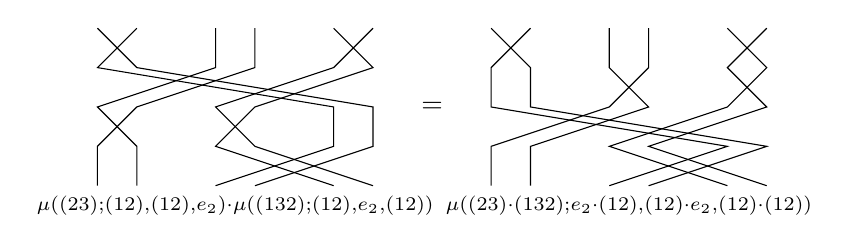
\begin{tikzpicture}[scale=0.5]
    \draw (1,0) -- (2,-1) -- (8,-2) -- (8,-3) -- (5,-4);
    \draw (2,0) -- (1,-1) -- (7,-2) -- (7,-3) -- (4,-4);
    \draw (4,0) -- (4,-1) -- (1,-2) -- (2,-3) -- (2,-4);
    \draw (5,0) -- (5,-1) -- (2,-2) -- (1,-3) -- (1,-4);
    \draw (7,0) -- (8,-1) -- (5,-2) -- (4,-3) -- (7,-4);
    \draw (8,0) -- (7,-1) -- (4,-2) -- (5,-3) -- (8,-4);
    %
    \node at (9.5,-2) {$=$};
    %
    \draw (11,0) -- (12,-1) -- (12,-2) -- (18,-3) -- (15,-4);
    \draw (12,0) -- (11,-1) -- (11,-2) -- (17,-3) -- (14,-4);
    \draw (14,0) -- (14,-1) -- (15,-2) -- (12,-3) -- (12,-4);
    \draw (15,0) -- (15,-1) -- (14,-2) -- (11,-3) -- (11,-4);
    \draw (17,0) -- (18,-1) -- (17,-2) -- (14,-3) -- (17,-4);
    \draw (18,0) -- (17,-1) -- (18,-2) -- (15,-3) -- (18,-4);
    %
    \node at (4.5,-4.5) {$\scriptstyle \mu\left((23);(12),(12), e_2\right) \cdot \mu\left((132); (12), e_2, (12)\right)$};
    \node at (14.5,-4.5) {$\scriptstyle \mu\left((23)\cdot (132); e_2 \cdot (12), (12) \cdot e_2, (12) \cdot (12)\right)$};
  \end{tikzpicture}
  \end{center}
\end{itemize}
\end{rem}

Action operads are themselves the objects of a category, $\mb{AOp}$. The morphisms of this category are defined below.
\begin{Defi}[(Map of action operads)]\label{Defi:mapaop}
A \textit{map of action operads} $f \colon  \Lambda \rightarrow \Lambda'$ consists of a map $f \colon \Lambda \rightarrow \Lambda'$ of the underlying operads such that
  \begin{enumerate}
    \item $\pi^{\Lambda'} \circ f = \pi^{\Lambda}$ (i.e., $f$ is a map of operads over $\Sigma$) and
    \item each $f_{n} \colon \Lambda(n) \rightarrow \Lambda'(n)$ is a group homomorphism.
  \end{enumerate}
\end{Defi}

\begin{prop}\label{prop:cat-of-aop}
There is a category with 
\begin{itemize}
\item objects the action operads $O$ in $\mb{Sets}$, 
\item morphisms as defined in \cref{Defi:mapaop},
\item identities $1_\Lambda \colon \Lambda \to \Lambda$ given by the identity morphism of $\Lambda$ as an operad,
and
\item composition given by composition of maps of operads.
\end{itemize}
\end{prop}

\begin{nota}[(The category of action operads)]\label{nota:cat_aop}
The category in \cref{prop:cat-of-aop} is called the \emph{category of action operads (in $\mb{Sets}$)}, and is denoted $\mb{AOp}$.
\end{nota}

\begin{prop}\label{prop:pi-in-aop}
Let $(\Lambda, \pi)$ be an action operad. The map $\pi \colon \Lambda \rightarrow \Sigma$ is a map of action operads.
\end{prop}


We now study some of the structure on the groups $\Lambda(n)$ for small values of $n$. Recall from \cref{nota:e_identity} that we write $e_{n}$ for the identity element in the group $\Lambda(n)$.
Many of our proofs rely on the following version of the Eckmann-Hilton argument.

\begin{prop}[(Eckmann-Hilton argument)]\label{prop:EH}
Let $G$ be a group with identity element $e$, and suppose $\varphi \colon G \times G \to G$ is a function. If $\varphi$ is a homomorphism, meaning that
\[
\varphi(g',h') \cdot \varphi(g,h) = \varphi(g' \cdot g, h' \cdot h),
\]
and $\varphi(g,e) = g = \varphi(e,g)$ for all elements $g \in G$, then 
\[
\varphi(g, h) = g \cdot h
\]
and $G$ is abelian.
\end{prop}

\begin{lem}\label{lem:calclem}
Let $\Lambda$ be an action operad.
\begin{enumerate}
\item In $\Lambda(1)$, the identity element for the group structure, $e_1$, is equal to the identity element for the operad structure, $\id$.
\item The equation
  \[
    \mu(e_{n}; e_{i_{1}}, \ldots, e_{i_{n}}) = e_{I}
  \]
holds for any natural numbers $n, i_{j}, I = \sum_{j=1}^n i_{j}$.
\item The group $\Lambda(1)$ is abelian.
\end{enumerate}
\end{lem}
\begin{proof}
For the first claim, we will prove that $\id \cdot e_1 = \id \cdot \id$, so $e_1 = \id$ by cancellation.
Note that since the only element of $\Sigma_1$ is the identity permutation, the action operad axiom \cref{eqn:ao_axiom} is
\[
\mu(g';f')\cdot \mu(g;f) = \mu(g'g; f'f)
\]
when $g, g' \in \Lambda(1)$.
Thus we obtain 
\begin{align*}
\id \cdot e_1 & = \mu(\id; \id) \cdot \mu(\id; e_{1}) \\
& = \mu(\id \cdot \id; \id \cdot e_{1}) \\
    &= \mu(\id \cdot \id; \id) \\
    &= \id \cdot \id
\end{align*}
using that $\id$ is the identity element for operadic multiplication, the $n=1$ action operad axiom explained above, that $e_1$ is the identity for group multiplication, and that $\id$ is the identity for operadic multiplication again.
Therefore $\id \cdot e_1 = \id \cdot \id$ as desired, and $e_1 = \id$.

%For the first claim, let $g \in \Lambda(1)$. Then
%  \begin{align*}
%    g & = g \cdot e_{1} \\
%    &= \mu(g; \id) \cdot \mu(\id; e_{1}) \\
%    &= \mu(g \cdot \id; \id \cdot e_{1}) \\
%    &= \mu(g \cdot \id; \id) \\
%    &= g \cdot \id
%  \end{align*}
%using that $e_{1}$ is the unit element for the group structure, that $\id$ is a two-sided unit for operad multiplication, and the final axiom for an action operad together with the fact that the only element of the symmetric group $\Sigma_{1}$ is the identity permutation. Thus $g = g \cdot \id$, so $\id = e_{1}$.

For the second claim, we write $\mu(e_{n}; e_{i_{1}}, \ldots, e_{i_{n}})$ as $\mu(e; \underline{e})$, and consider the square of this element. We find that
  \begin{align*}
    \mu(e; \underline{e}) \cdot \mu(e; \underline{e}) & = \mu(e \cdot e; \underline{e} \cdot \underline{e}) \\
    &= \mu(e; \underline{e}),
  \end{align*}
where the first equality follows from the last action operad axiom together with the fact that $e$ gets mapped to the identity permutation; here $\underline{e} \cdot \underline{e}$ is the sequence $e_{i_{1}} \cdot e_{i_{1}}, \ldots, e_{i_{n}} \cdot e_{i_{n}}$. Thus $\mu(e; \underline{e})$ is an idempotent element of the group $\Lambda(I)$, so must be the identity element $e_{I}$.

For the final claim, note that the specific operadic multiplication map $\mu \colon \Lambda(1) \times \Lambda(1) \rightarrow \Lambda(1)$ is a group homomorphism following from the action operad axioms, and $\id = e_{1}$ is a two-sided unit, so \cref{prop:EH} shows that $\mu$ is actually group multiplication and that $\Lambda(1)$ is abelian.
\end{proof}

\begin{lem}\label{lem:G0abel}
Let $\Lambda$ be an action operad. For any $g, h \in \Lambda(0)$, the equation
\[
g \cdot h = \mu(e_2; g,h)
\]
holds. As a consequence, $\Lambda(0)$ is abelian.
\end{lem}
\begin{proof}
The function $\Lambda(0) \times \Lambda(0) \to \Lambda(0)$ given by
\[
g, h \mapsto \mu(e_2; g, h)
\]
is a group homomorphism by the action operad axiom \cref{eqn:ao_axiom} as we verify below.
\[
\mu(e_2; g', h') \cdot \mu(e_2; g, h) = \mu(e_2 \cdot e_2; g' \cdot g, h' \cdot h) = \mu(e_2; g' \cdot g, h' \cdot h)
\]
In order to apply \cref{prop:EH} and conclude that $g \cdot h = \mu(e_2; g, h)$, we must verify that 
\[
\mu(e_2; e_0, g) = g = \mu(e_2; g, e_0)
\]
for all $g \in \Lambda(0)$.
We will prove the first equality and leave the second to the reader, as it follows in a similar fashion.

By the identity axiom for an operad and the first part of \cref{lem:calclem}, we have $g = \mu(\id; g) = \mu(e_1; g)$ for any $g \in \Lambda(0)$.
By the second part of \cref{lem:calclem}, we also have the equality $e_1 = \mu(e_2; e_0, e_1)$.
Then
  \begin{align*}
   g & = \mu(e_1; g) \\
    &= \mu(\mu(e_2; e_0, e_1); g) \\
    & = \mu(\mu(e_2; e_0, e_1); \mu(e_1; g)) \\
    & = \mu(e_2; e_0, g),
  \end{align*}
  where the final equality follows from operadic associativity together with $g = \mu(e_1; g)$.
  This calculation shows $g = \mu(e_2; e_0, g)$ as desired, and thus proves that the function $\mu(e_2; -,-)$ satisfies the hypotheses in \cref{prop:EH}.
  Therefore $g \cdot h = \mu(e_2; g,h)$ and $\Lambda(0)$ is abelian.
%  Note first that
%    \begin{align*}
%      \mu(e_2; g, h) &= \mu(e_2 \cdot e_2; g \cdot e_0, e_0 \cdot h) \\
%      &= \mu(e_2; g, e_0) \cdot \mu(e_2; e_0, h),
%    \end{align*}
%  so for the first claim that $\mu(e_2; g, h) = g \cdot h$ it will suffice to show that $\mu(e_2; g, e_0) = g$ and $\mu(e_2; e_0, h) = h$ for all $g, h \in \Lambda(0)$. We will use the fact that $\mu(e_0; ) = e_0$, which follows below from a similar argument found in the second part of \cref{calclem}.
%    \begin{align*}
%      \mu(e_0;)\mu(e_0;) &= \mu\left(e_0^2;\right) \\
%      &= \mu(e_0;).
%    \end{align*}
%  Since $\mu(e_0;)$ is an idempotent element of $\Lambda(0)$, then it must be the identity $e_0$. Now we have this, the following sequence of calculations shows that $\mu(e_2; g, e_0) = g$, while a similar calculation would show that $\mu(e_2; e_0, h) = h$. Using \cref{calclem},
%    \begin{align*}
%      g &= \mu(e_1; g) \\
%      &= \mu(\mu(e_2; e_0, e_1); g) \\
%      &= \mu(e_2; \mu(e_0;), \mu(e_1; g)) \\
%      &= \mu(e_2; e_0, g).
%    \end{align*}
%  It remains to show that $\Lambda(0)$ is abelian, which relies on the coincidence of the operad multiplication and the group operation in $\Lambda(0)$, in an Eckmann-Hilton style argument.
%    \begin{align*}
%      g \cdot h &= \mu(e_2; g, h) \\
%      &= \mu(e_2 \cdot e_2; e_0 \cdot g, h \cdot e_0) \\
%      &= \mu(e_2; e_0, h) \cdot \mu(e_2; g, e_0) \\
%      &= h \cdot g.
%    \end{align*}
\end{proof}

The symmetric operad structure on the symmetric groups in \cref{ex:Sigma} was constructed using the functions $\beta, \delta$ from \cref{Defi:beta-s} and \cref{Defi:delta-s}, respectively.
We are now ready to show that any action operad can be described in this way, as promised in the introductory remarks to this section.

%Note that the operad of symmetric groups $\Sigma$ has its action operad structure determined by two auxiliary operations, which we have previously used to describe particular types of operadic composition as described in \cref{conv1} \eqref{conv:beta_delta} and \cref{exSigma}. Rather than simply being convenient notation for common occurences of operadic composition, we will use these ideas to give a characterisation of action operads. First we recall these notions in more detail in the case of the symmetric operad $\Sigma$. The first operation is the block sum of permutations which we denote by
%  \[
%    \beta \colon \Sigma_{k_{1}} \times \cdots \times \Sigma_{k_{n}} \rightarrow \Sigma_{K},
%  \]
%where $K = \sum k_{i}$. The second is a kind of diagonal map which is defined for any natural number $n$ together with natural numbers $k_{1}, \ldots, k_{n}$. Then
%  \[
%    \delta = \delta_{n; k_{1}, \ldots, k_{n}} \colon \Sigma_{n} \rightarrow \Sigma_{K},
%  \]
%is defined on $\sigma \in \Sigma_{n}$ by permuting the elements $1, 2, \ldots, k_{1}$ together in a block according to the action of $\sigma \in \Sigma_{n}$ on $1$, then $k_{1}+1, \ldots, k_{1}+k_{2}$ together in a block according to the action of $\sigma$ on $2$, and so on. The first of these, $\beta$, is a group homomorphism, while $\delta$ is a sort of twisted homomorphism, and taken together they define operadic multiplication in $\Sigma$.

% \begin{Defi}\label{Defi:aop_bl}
% Let $\Lambda$ be an action operad. For $h_i \in \Lambda(k_i)$ and $g \in \Lambda(n)$, define
%   \begin{align*}
%     \beta(h_{1}, \ldots, h_{n}) &= \mu(e_n; h_{1}, \ldots, h_{n}), \\
%     \delta_{n; k_{1}, \ldots, k_{n}}(g) &= \mu(g; e_{k_1}, \ldots, e_{k_n}).
%   \end{align*}
% \end{Defi}


\begin{thm}\label{thm:charAOp}
An action operad $\Lambda$ determines, and is uniquely determined by, the following: 
\begin{itemize}
\item groups $\Lambda(n)$ together with group homomorphisms $\pi_{n} \colon \Lambda(n) \rightarrow \Sigma_{n}$,
\item a group homomorphism
  \[
    \Lambda(k_{1}) \times \cdots \times \Lambda(k_{n}) \stackrel{\beta}{\longrightarrow} \Lambda(k_{1} + \cdots + k_{n}),
  \]
for each $n > 0$ and $k_{1}, \ldots, k_{n}$\ngnote{Used to have: together with the degenerate case of $n=0$ which then is a group homomorphism $1 \rightarrow \Lambda(0)$. Do we need this?}, and
\item a function of sets
  \[
    \Lambda(n) \stackrel{\delta_{n; k_{1}, \ldots, k_{n}}}{\longrightarrow} \Lambda(k_{1} + \cdots + k_{n})
  \]
for each $n, k_{1}, \ldots, k_{n}$,
\end{itemize}
subject to the axioms below. In what we write below, we use the following notational conventions.
\begin{itemize}
\item The symbols $f,g,h$, with or without subscripts, always refer to an element of some group $\Lambda(n)$.
\item The symbols $j,k,m,n,p$ are all natural numbers, and $i$ is a natural number between 1 and $n$.
\end{itemize}
Axioms:
\begin{enumerate}
\item\label{eq1} The homomorphisms $\beta$ are natural with respect to the maps $\pi_{n}$, where $K = k_{1} + \cdots + k_{n}$.
  \[
    \xy
      (0,0)*+{\Lambda(k_{1}) \times \cdots \times \Lambda(k_{n}) } ="00";
      (0,-15)*+{\Sigma_{k_{1}} \times \cdots \times \Sigma_{k_{n}}  } ="01";
      (40,0)*+{\Lambda(K) } ="20";
      (40,-15)*+{\Sigma_{K} } ="21";
      {\ar^{\beta} "00" ; "20"};
      {\ar^{\pi} "20" ; "21"};
      {\ar_{\pi_1 \times \cdots \times \pi_n} "00" ; "01"};
      {\ar_{\beta} "01" ; "21"};
    \endxy
  \]

\item\label{eq2} The homomorphism $\beta \colon \Lambda(k) \rightarrow \Lambda(k)$ is the identity.
\item\label{eq3} The homomorphisms $\beta$ are associative in the sense that the equation
% \[
% \beta(h_{11}, \ldots, h_{1j_{1}}, h_{21}, \ldots, h_{2j_{2}}, \ldots, h_{nj_{n}}) = \beta\left( \beta(h_{11}, \ldots, h_{1j_{1}}), \ldots, \beta(h_{n1}, \ldots, h_{nj_{n}}) \right)
% \]
\[
  \beta(\underline{h_1},\ldots,\underline{h_n}) = \beta(\beta(\underline{h_1}),\ldots,\beta(\underline{h_n}))
\]
holds, where $\underline{h_i} = h_{i1},\ldots,h_{ij_i}$.
\item\label{eq4} The functions $\delta_{n; k_{1}, \ldots, k_{n}}$ are natural with respect to the maps $\pi_{n}$, where $K = k_1 + \cdots + k_n$.
  \[
    \xy
      (0,0)*+{\Lambda(n)} ="00";
      (40,0)*+{\Lambda(k_{1} + \cdots + k_{n}) } ="20";
      (0,-15)*+{\Sigma_{n}  } ="01";
      (40,-15)*+{\Sigma_{k_{1} + \cdots + k_{n}} } ="21";
      {\ar^{\delta} "00" ; "20"};
      {\ar^{\pi} "20" ; "21"};
      {\ar_{\pi} "00" ; "01"};
      {\ar_{\delta} "01" ; "21"};
    \endxy
  \]


\item\label{eq5} The function $\delta_{n; 1, \ldots, 1} \colon \Lambda(n) \rightarrow \Lambda(n)$ is the identity. The function $\delta_{1;n} \colon \Lambda(1) \to \Lambda(n)$ maps $e_1$ to $e_n$\ngnote{I think something more general is true: any $\delta$ maps $e_n$ to $e_K$}.

\item\label{eq6} The equation $\delta_{n; k_1, \ldots, k_n}(g) \delta_{n; j_1, \ldots, j_n}(h) = \delta_{n; j_1,\ldots,j_n}(gh)$ holds when

  \[
    k_{i} = j_{h^{-1}(i)}.
  \]
\item\label{eq7} The functions $\delta$ are associative in the sense that the equation
% \[
% \delta_{m_1 + \cdots + m_n; p_{11}, \ldots, p_{1m_{1}}, p_{21}, \ldots, p_{nm_{n}}}\left( \delta_{n; m_{1}, \ldots, m_{n}}(f) \right) = \delta_{n; P_{1}, \ldots, P_{n}}(f)
% \]
  \[
    \delta_{m_1 + \cdots + m_n; \underline{p_1},\ldots,\underline{p_n}}\left( \delta_{n; m_{1}, \ldots, m_{n}}(g) \right) = \delta_{n; P_{1}, \ldots, P_{n}}(g)
  \]
holds, where $P_{i} = p_{i1} + \cdots + p_{im_{i}}$ and $\underline{p_i} = p_{i1}, \ldots, p_{im_i}$.
\item\label{eq8} The equation
  \[
    \delta_{n;k_1,\ldots,k_n}(g) \beta(h_{1}, \ldots, h_{n}) = \beta(h_{g^{-1}(1)}, \ldots,  h_{g^{-1}(n)}) \delta_{n;k_{g^{-1}(1)},\ldots,k_{g^{-1}(n)}}(g)
  \]
holds, where $h_{i} \in \Lambda(k_{i})$.
\item\label{eq9} The equation
  \[
    \beta(\delta_{1}(g_{1}), \ldots, \delta_{n}(g_{n})) = \delta_{c}(\beta(g_{1}, \ldots, g_{n}))
  \]
holds, where $\delta_{i}(g_{i})$ is shorthand for $\delta_{k_{i}; m_{i1}, \ldots, m_{ik_{i}}}(g_{i})$ and $\delta_{c}$ is shorthand for
  \[
    \delta_{k_{1}+\cdots + k_{n}; m_{11}, m_{12}, \ldots, m_{1k_{1}}, m_{21}, \ldots, m_{nk_{n}}}.
  \]
\end{enumerate}
\end{thm}

\begin{proof}
Let $\Lambda$ be an action operad, and define 
\begin{align*}\label{eqn:bd-from-aop}
\beta(g_1, \ldots, g_n) & = \mu(e_n; g_1, \ldots, g_n),\\
\delta_{n; k_1, \ldots, k_n}(g) & = \mu(g; e_{k_1}, \ldots, e_{k_n}).
\end{align*}
Since $\pi \colon \Lambda \rightarrow \Sigma$ is an operad map, Axioms \ref{eq1} and \ref{eq4} hold by the definition of the operad structure on $\Sigma$ in \cref{ex:Sigma}. 
Since $\Lambda$ is an operad of sets, Axioms \ref{eq2} and \ref{eq5} follow from the operad unit axioms and the first part of \cref{lem:calclem}, and Axioms \ref{eq3}, \ref{eq7}, and \ref{eq9} follow from the operad associativity axiom and the second part of \cref{lem:calclem}. Axioms \ref{eq6} and \ref{eq8} are special cases of the additional action operad axiom, as is the fact that $\beta$ is a group homomorphism.

Conversely, given the data above, we need only define the operad multiplication, verify the operad unit and multiplication axioms, and finally check the action operad axiom. Multiplication is given by
  \[
    \mu(g; h_{1}, \ldots, h_{n}) = \delta_{n; k_{1}, \ldots, k_{n}}(g) \beta(h_{1}, \ldots, h_{n})
  \]
where $h_{i} \in \Lambda(k_{i})$. The identity element $\id$ for the operad structure is $e_1 \in \Lambda(1)$.

We now verify the operad unit axioms. Let $g, h \in \Lambda(n)$. Then
  \begin{align*}
    \mu(e_1; g) &= \delta(e_1)\beta(g) \\
    &= e_1 \cdot g \\
    &= g, \\
    \mu(h; e_1, \ldots, e_1) &= \delta_{n; 1, \ldots, 1}(h)\beta(e_1, \ldots, e_1) \\
    &= h \cdot e_n \\
    &= h
  \end{align*}
by Axioms \ref{eq2} and \ref{eq5}, together with the fact that $\beta$ is a group homomorphism.
Thus $e_1$ satisfies the identity axioms for operadic multiplication.

For the operad associativity axiom, let
\begin{itemize}
\item $f \in \Lambda(m),$
\item $g_{i} \in \Lambda(n_{i})$ for $i=1, \ldots, m$, and
\item $h_{ij} \in \Lambda(p_{i,j})$ for $i=1, \ldots, m$ and $j=1, \ldots, n_{i}$.
\end{itemize}
Further, let $P_{i} = p_{i1} + \cdots + p_{in_{i}}$ and $\underline{h_i}$ denote the list $h_{i1}, h_{i2}, \ldots, h_{in_{i}}$. We must then show that
  \[
    \mu\big( f; \mu(g_{1}; \underline{h_1}), \ldots, \mu(g_{m}; \underline{h_m}) \big) = \mu\big( \mu(f; g_{1}, \ldots, g_{m}); \underline{h_1}, \ldots, \underline{h_m} \big).
  \]
By definition, the left side of this equation is
  \[
    \delta_{m; P_{1}, \ldots, P_{m}}(f) \beta\big( \mu(g_{1}; \underline{h_1}), \ldots, \mu(g_{m}; \underline{h_m}) \big),
  \]
and
  \[
    \mu\left(g_{i}; \underline{h_i}\right) = \delta_{n_{i}; p_{i1}, \ldots, p_{in_{i}}}(g_{i})\beta\left(h_{i1}, \ldots, h_{in_{i}}\right).
  \]
From this point, we suppress subscripts on the $\delta$'s.
Since $\beta$ is a group homomorphism, we can then rewrite the left side as
  \[
    \delta(f)\beta\big(\delta(g_{1}), \ldots, \delta(g_{m})\big)\beta\big(\beta(\underline{h_1}), \ldots, \beta(\underline{h_m})\big)
  \]
where we have suppressed the subscripts on the $\delta$'s. By Axiom \ref{eq3},
  \[
    \beta\big(\beta(\underline{h_1}), \ldots, \beta(\underline{h_m})\big) = \beta\left(\underline{h_1},\ldots,\underline{h_m}\right).
  \]
Furthermore, Axiom \ref{eq9} above shows that
  \[
    \beta\big(\delta(g_{1}), \ldots, \delta(g_{m})\big) = \delta\big(\beta(g_{1}, \ldots, g_{m})\big).
  \]
Thus we have shown that the left side of the operad associativity axiom is equal to
  \[
    \delta(f)\delta\big(\beta(g_{1}, \ldots, g_{m})\big)\beta\left(\underline{h_1},\ldots,\underline{h_m}\right).
  \]
Now the right side is
  \[
    \mu\big( \mu (f; g_{1}, \ldots, g_{m}); \underline{h_1}, \ldots, \underline{h_m} \big),
  \]
which is by definition
  \[
    \delta\big(\mu (f; g_{1}, \ldots, g_{m})\big)\beta\left(\underline{h_1}, \ldots, \underline{h_m}\right).
  \]
Cancelling the $\beta\left(\underline{h_1}, \ldots, \underline{h_m}\right)$ terms, verifying the operad associativity axiom reduces to showing
\begin{eqn}\label{eqn:opass}
\delta(f)\delta\big(\beta(g_{1}, \ldots, g_{m})\big) = \delta\big(\mu (f; g_{1}, \ldots, g_{m})\big).
\end{eqn}
By the definition of $\mu$,
  \[
    \delta\big(\mu (f; g_{1}, \ldots, g_{m})\big) = \delta\big(\delta(f)\beta(g_{1}, \ldots, g_{m}) \big)
  \]
which is itself equal to
\begin{eqn}\label{eqn:opass2}
\delta\big(\delta(f)\big) \delta\big(\beta(g_{1}, \ldots, g_{m})\big)
\end{eqn}
by Axiom \ref{eq6} above. 
Now the $\delta(f)$ on the left side of \cref{eqn:opass} uses $\delta_{n; P_{1}, \ldots, P_{n}}$, while the $\delta(\delta(f))$ in \cref{eqn:opass2} is actually
  \[
    \delta_{m_1 + \cdots + m_{n}; q_{ij}}(\delta_{n; m_{1}, \ldots, m_{n}} (f))
  \]
where the $q_{ij}$ are defined, by Axiom \ref{eq6}, to be given by
  \[
    q_{ij} = p_{i,g_{i}^{-1}(j)}
  \]
using the compatibility of $\beta$ and $\pi$ in Axiom \ref{eq1}. By Axiom \ref{eq7}, this composite of $\delta$'s  is then $\delta_{n; Q_{1}, \ldots, Q_{n}}$ where $Q_{i} = q_{i1} + \cdots + q_{im_{i}}$. But by the definition of the $q_{ij}$, we immediately see that $Q_{i} = P_{i}$, so the $\delta(f)$ in \cref{eqn:opass} is equal to the $\delta(\delta(f))$ appearing in \cref{eqn:opass2}, concluding the proof of the operad associativity axiom.

Writing $\mu(g;\underline{h}) = \mu\left(g; h_{1}, \ldots, h_{n}\right)= $ and $\mu(g';\underline{h'}) = \mu\left(g'; h_{1}', \ldots, h_{n}'\right)$, the action operad axiom is now the calculation below, and uses Axioms \ref{eq4} and \ref{eq8}.
\begin{small}
  \begin{align*}
    \mu(g;\underline{h})\mu(g';\underline{h'}) &= \delta\left(g\right) \beta\left(h_{1}, \ldots, h_{n}\right) \delta\left(g'\right) \beta\left(h_{1}', \ldots, h_{n}'\right) \\
    &= \delta\left(g\right) \delta\left(g'\right) \beta\left(h_{g'(1)}, \ldots, h_{g'(n)}\right)  \beta\left(h_{1}', \ldots, h_{n}'\right) \\
    &= \delta\left(gg'\right) \beta\left(h_{g'(1)}h_{1}', \ldots, h_{g'(n)}h_{n}'\right) \\
    &= \mu\left(gg'; h_{g'(1)}h_{1}', \ldots, h_{g'(n)}h_{n}'\right)
  \end{align*}
\end{small}
\end{proof}

\begin{prop}[Corollary 2.17,  \cite{zhang-grp}]\label{prop:surjortriv} Let $\Lambda$ be an action operad. Then the homomorphisms $\pi_n \colon \Lambda(n) \rightarrow \Sigma_n$ are either all surjective or all the zero map.
\end{prop}
\begin{proof}
% QQQ New short snazzy proof: It's basically the same, but the \beta and \delta axioms allow it to go through a bit more cleanly and less `handwavy'.
We will prove each case separately. The two cases coincide for $n = 0, 1$ as both $\Sigma_0, \Sigma_1$ are the trivial group and therefore any homomorphism with one of them as its codomain is both surjective and the zero map. Since $\Sigma_2$ only has one non-identity element, any homomorphism $G \rightarrow \Sigma_2$ must necessarily be surjective or the zero map.

Suppose that $\pi_2 \colon \Lambda(2) \rightarrow \Sigma_2$ is surjective, so there exists $g \in \Lambda(2)$ such that $\pi_2(g) = \trans{1}{2}$. Let $n>2$. Since $\Sigma_n$ is generated by the adjacent transpositions $\trans{a}{a+1}$, we will show that each such element is in the image of $\pi_n$. Write $\underline{x}^i$ for the $i$-tuple $x, x, \ldots, x$. Then $\trans{a}{a+1} = \beta(\underline{e_1}^{a-1} ,\trans{1}{2},\underline{e_1}^{n-a-1})$ in $\Sigma$, so
  \begin{align*}
      \trans{a}{a+1} &= \beta(\underline{e_1}^{a-1},\trans{1}{2},\underline{e_1}^{n-a-1}) \\ &= \beta(\underline{\pi_1(e_1)}^{a-1},\pi_2(g),\underline{\pi_1(e_1)}^{n-a-1}) \\
      &= \pi_n(\beta(\underline{e_1}^{a-1},g,\underline{e_1}^{n-a-1}))
  \end{align*}
by Axiom \ref{eq1} of \ref{thm:charAOp}.
Thus $\pi_n$ is surjective for all $n>2$ if $\pi_2$ is surjective.

Now we will consider the case where $\pi_2$ is the zero map.
Suppose that there exists $g \in \Lambda(n)$ such that $\pi_n(g) = \sigma \neq e_n$ in $\Sigma_n$.
Then we can find $1 \leq i < j \leq n$ such that $\sigma(j) < \sigma(i)$.
Consider the element 
\[
h = \delta_{n; \underline{0}^{i-1}, 1, \underline{0}^{j-i-1}, 1, \underline{0}^{n-j}}(g) \in \Lambda(2).
\]
By the assumption that $\pi_2$ is the zero map, we must have that $\pi_2(h) = e_2$, but by Axiom \ref{eq4} of \ref{thm:charAOp} we also compute
\[
\pi_2(h) = \delta_{n; \underline{0}^{i-1}, 1, \underline{0}^{j-i-1}, 1, \underline{0}^{n-j}}\big( \pi_n(g) \big) =  \delta_{n; \underline{0}^{i-1}, 1, \underline{0}^{j-i-1}, 1, \underline{0}^{n-j}}\big( \sigma \big).
\]
The element $\delta_{n; \underline{0}^{i-1}, 1, \underline{0}^{j-i-1}, 1, \underline{0}^{n-j}}\big( \sigma \big)$ is equal to $\trans{1}{2}$ by the choice of $i, j$ and \cref{Defi:delta-s}.
These two computations of $\pi_2(h)$ are in contradiction, so there must be no such $g \in \Lambda(n)$.
Thus if $\pi_2$ is the zero map, so is $\pi_n$ for all $n>2$.
%
%
%Assume that $\pi_n$ is zero for some $n \geq 2$. Now let $\sigma \in \operatorname{Im} \pi_{n+1}$, so there exists $g \in \Lambda(n+1)$ such that $\pi_{n+1}(g) = \sigma$. Now $\delta_{n+1;\underline{1},0,\underline{1}}(\sigma)$ is an element of $\Sigma_n$ and
%  \begin{align*}
%    \delta_{n+1;\underline{1},0,\underline{1}}(\sigma) &= \delta_{n+1;\underline{1},0,\underline{1}}(\pi_{n+1})(g) \\
%    &= \pi_n(\delta_{n+1;\underline{1},0,\underline{1}}(g)) \\
%    &= e_n,
%  \end{align*}
%using Axiom \ref{eq4} of \ref{thm:charAOp}. Hence $\sigma = e_{n+1}$ or $\sigma = \trans{a}{a+1}$.
%
%If $\sigma = e_{n+1}$ then $\pi_{n+1}$ is zero. But if $a \neq 1$, then using Axiom \ref{eq4} again
%  \begin{align*}
%    \trans{a-1}{a} &= \delta_{n+1;0,\underline{1}}(\trans{a}{a+1}) \\
%    &= \delta_{n+1;0,\underline{1}}(\pi_{n+1}(g)) \\
%    &= \pi_n(\delta_{n+1;0,\underline{1}}(g)) \\
%    &= e_n,
%  \end{align*}
%a contradiction. If $a = 1$, then $\trans{a}{a+1} = \trans{1}{2}$ and again using Axiom \ref{eq4}
%  \begin{align*}
%    \trans{1}{2} &= \delta_{n+1;\underline{1},0}(\trans{a}{a+1}) \\
%    &= \delta_{n+1;\underline{1},0}(\pi_{n+1}(g)) \\
%    &= \pi_n(\delta_{n+1;\underline{1}}(g),0) \\
%    &= e_n,
%  \end{align*}
%again a contradiction. Hence $\sigma = e_{n+1}$ and so the image of $\pi_{n+1}$ is trivial.

% QQQ Old long proof:
% We will prove each case separately. The two cases coincide for $n = 0$ and $n = 1$ as $\pi_0$ and $\pi_1$ are both the zero map and since $\Sigma_0$ and $\Sigma_1$ are the trivial group then these maps are also surjective.

% Any homomorphism $G \rightarrow \Sigma_2$ must necessarily be surjective or the zero map. To begin we will show that if $\pi_2 \colon \Lambda(2) \rightarrow \Sigma_2$ is surjective then, by induction, the rest of the maps $\pi_n$ are also surjective. If $\pi_2$ is surjective then there exists an element $g_{1,1} \in \Lambda(2)$ such that $\pi_2(g_{1,1}) = \trans{1}{2}$. Now assume that for some $j \geq 2$ that $\pi_j$ is surjective. In particular, this means that for each transposition $\trans{a}{a+k} \in \Sigma_j$, where $1 \leq a \leq j-1$ and $a + k \leq j$, there exists $g_{a,k} \in \Lambda(j)$ such that $\pi_j(g_{a,k}) = \trans{a}{a+k}$. We will use these assumptions to show that each transposition in $\Sigma_{j+1}$ can be written as the image under $\pi_{j+1}$ of some element in $\Lambda(j+1)$, hence any permutation in $\Sigma_{j+1}$ can similarly be written.


% Let $\trans{a}{a+k} \in \Sigma_j$, where $1 \leq a \leq j$ and $a + k \leq j+1$. If $a + k \leq j$, then $\trans{a}{a+k} = \trans{a}{a+k}(j + 1) \in \Sigma_{j+1}$. This transposition can be written as
%   \begin{align*}
%     \trans{a}{a+k} &= \mu^{\Sigma}(e_2 ; \trans{a}{a+k}, e_1) \\
%               &= \mu^{\Sigma}(\pi_2(e_2); \pi_j(g_{a,k}), \pi_1(e_1)) \\
%               &= \pi_{j+1}\left(\mu^{\Lambda}(e_2; g_{a,k},e_1)\right).
%   \end{align*}
% Similarly, if $a > 1$ then this transposition can be written as
%   \begin{align*}
%    \trans{a}{a+k} &= \mu^{\Sigma}(e_2 ; e_1, \trans{a-1}{a+k-1}) \\
%               &= \mu^{\Sigma}(\pi_2(e_2); \pi_1(e_1), \pi_j(g_{a-1,k})) \\
%               &= \pi_{j+1}\left(\mu^{\Lambda}(e_2; e_1, g_{a-1,k})\right).
%   \end{align*}
% Finally, if $a = j$ and $k = 1$, then $\trans{a}{a+k} = \trans{j}{j+1}$. This can be written as
%   \begin{align*}
%     (j \,\,\, j + 1) &= \mu^{\Sigma}(e_2 ; e_{j-1}, (1 \,\,\, 2)) \\
%               &= \mu^{\Sigma}(\pi_2(e_2); \pi_{j-1}(e_{j-1}), \pi_2(g_{1,1})) \\
%               &= \pi_{j+1}\left(\mu^{\Lambda}(e_2; e_{j-1}, g_{1,1})\right).
%   \end{align*}
% Hence $\pi_{j+1}$ is surjective and so all $\pi_n$ are surjective.

% Now instead suppose that $\pi_2 \colon \Lambda(2) \rightarrow \Sigma_2$ is the zero map. Assume that $\pi_j \colon \Lambda(j) \rightarrow \Sigma_j$ is the zero map for some $j \geq 2$. Letting $\sigma \in \textrm{Im}\,\pi_{j+1}$, there exists $g \in \Lambda(j+1)$ such that $\pi_{j+1}(g) = \sigma$. We can then consider the elements $\mu^\Sigma(\sigma; \underline{e_1}, e_o, \underline{e_1})$ where $\underline{e_1}$ means a sequence of $e_1$'s and with $e_0$ in the $k$th position, with $1 \leq k \leq j + 1$. Now
%   \begin{align*}
%     \mu^\Sigma(\sigma; \underline{e_1}, e_o, \underline{e_1}) &= \mu^\Sigma(\pi_{j+1}(g); \underline{\pi_1(e_1)}, \pi_0(e_0), \underline{\pi_1(e_1)}) \\
%     &= \pi_j(\mu^\Lambda(g; \underline{e_1}, e_0, \underline{e_1})) \\
%     &= e_j.
%   \end{align*}
% We can think of this permutation as being $\sigma$ with the $k$th string removed - in \cref{rem:crossed} we comment on such `face' and `degeneracy' maps as used here, and see \cite{ber-simplicial} for a more careful treatment of this idea. Now each of these is the identity $e_j$, as shown above. This means that $\sigma$ must either have been the identity $e_{j+1}$ or a transposition of the form $\trans{a}{a+1}$, where $1 \leq a \leq j$.

% If $\sigma$ is the identity $e_{j+1}$, then we are done since this would give $\textrm{Im}\,\pi_{j+1} = \{e_{j+1}\}$. Instead suppose that $\sigma = \trans{a}{a+1} \in \Sigma_{j + 1}$. Then if $1 < a \leq j$ we can use this to give
%   \begin{align*}
%     \trans{a-1}{a} &= \mu^\Sigma(\trans{a}{a+1}; e_0, \underline{e_1}) \\
%     &= \mu^\Sigma(\pi_{j+1}(g);\pi_0(e_0), \underline{\pi_1(e_1)}) \\
%     &= \pi_j(\mu^\Lambda(g; e_0, \underline{e_1})) \\
%     &= e_j.
%   \end{align*}
% This gives a contradiction, hence $\sigma \neq \trans{a}{a+1}$ and must be the identity $e_{j+1}$.

% Similarly, if $\sigma = \trans{1}{2} \in \Sigma_{j+1}$, then in $\Sigma_j$ we find that
%   \begin{align*}
%     \trans{1}{2} &= \mu^\Sigma(\trans{1}{2} ; \underline{e_1}, e_0) \\
%     &= \mu^\Sigma(\pi_{j+1}(g); \underline{\pi_1(e_1)}, \pi_0(e_0)) \\
%     &= \pi_j(\mu^\Lambda(g ; \underline{e_1}, e_0)) \\
%     &= e_j.
%   \end{align*}
% Again, a contradiction, hence $\sigma = e_{j+1}$.
\end{proof}



\section{Examples}\label{sec:aop-examples}

In this section, we expand our collection of examples  and non-examples of action operads. 
In all but one case, \cref{ex:abgp-aop}, the examples we provide have appeared elsewhere.
The non-examples we provide were largely sourced from questions received after preliminary talks on this research by the authors. 

\begin{example}[(Action operad of braid groups)]\label{example:aop-braid}
One can form an operad $B$ where $B(n)$ is the underlying set of the $n$th braid group, $B_{n}$.
We define the operad structure using the functions $\beta, \delta$ from \cref{rem:br-op-needed}.
Yau checks that these groups and functions satisfy the axioms of an action operad in \cite[Prop 5.2.5]{yau_infinity_2021}, but we note that each of the nine axioms in \cref{thm:charAOp} follows immediately by using the geometric definitions of $\beta, \delta$.
%
%
%Copied:
%
%In order to make sense of this definition, we must define $\beta(\tau_1,\ldots,\tau_n)$ and $\delta(\sigma)$ in the context of braids. The first is the block sum in the obvious sense:  given $n$ different braids on $k_{1}, \ldots, k_{n}$ strands, respectively, we form a new braid on $k_{1} + \cdots + k_{n}$ strands by taking a disjoint union where the braid $\tau_{i}$ is to the left of $\tau_{j}$ if $i < j$. The braid $\delta(\sigma)$ is obtained by replacing the $i$th strand with $k_{i}$ consecutive strands, all of which are braided together according to $\sigma$. These operations are sometimes referred to as `cabling' operations for braids, as described in, for example, \cite{doucot_local_2025}.
%
%Copied 2:
%
%One can form an operad $B$ where $B(n)$ is the underlying set of the $n$th braid group, $B_{n}$. This is done in much the same way as we did for the symmetric operad using the `cabling' operations for braids described after \cref{broperad}. The collections of maps $\pi_{n} \colon B_{n} \rightarrow \Sigma_{n}$ giving the underlying permutation of each braid constitutes an operad map (of non-symmetric or braided operads) operads $Br \rightarrow \Sigma$.
\end{example}

\begin{Defi} For each $n \in \mathbb{N}$, the \emph{ribbon braid group} $RB_{n}$ is the group whose presentation is the same as that of the braid group $B_{n}$, except with the addition of $n$ new generators $t_1, \ldots, t_n$, known as the \emph{twists}. These twists all commute with one other, and also commute with all braids except in the following cases:
  \begin{align*}
    b_i \cdot t_i &= t_{i+1} \cdot b_i,\\
    b_i \cdot t_{i+1} &= t_i \cdot b_i.
  \end{align*}
The \emph{ribbon braid operad} $RB$ is then the operad made up of these groups in a way that extends the definition of the braid operad. In other words, the identity is still $e_1 \in RB_1$, and the operadic multiplication is built up in stages in exactly the same ways as in \cref{broperad}, but with some additional rules for dealing with twists. With regards to the tensor product, we have that for any twist $t_i \in RB_{n}$,
  \[
    t_i = e_{i-1} \otimes t \otimes e_{n-i}
  \]
where $t$ is the sole twist in $RB_1$, and for the `block twists' $t_{(m)}$ we again work recursively:
  \[
    t_{(0)} = e_n, \quad \quad \quad t_{(m+m')} = \left(t_{(m)} \otimes t_{(m')}\right) \cdot b_{(m', m)} \cdot b_{(m, m')}
  \]
\end{Defi}

Much as the symmetric groups can be represented by crossings of a collection of strings, and the braid groups by braidings of strings, the ribbon braid groups deal with the ways that one can braid together several flat ribbons, including the ability to twist a ribbon about its own axis by 360 degrees. The actual definition of the ribbon braid groups is as the fundamental group of a configuration space in which points have labels in the circle, $S^{1}$; see \cite{sal-wahl}.
\begin{center} \begin{tabular}{ccc}
			\begin{tikzpicture}[baseline]
				\node(xl1) at (-0.7,1){};
				\node(xr1) at (-0.3,1){};
				\node(yl1) at (0.3,1){};
				\node(yr1) at (0.7,1){};
				\node(yl2) at (-0.7, -1){};
				\node(yr2) at (-0.3, -1){};
				\node(xl2) at (0.3, -1){};
				\node(xr2) at (0.7, -1){};
				\node(b) at (0,0)[circle,fill=white, minimum size=0.5cm]{};
       				\draw[rounded corners](xl1.north) to (-0.7,0.5) to (0.3,-0.5) to (xl2.south);
       				\draw[rounded corners](xr1.north) to (-0.3,0.5) to (0.7,-0.5) to (xr2.south);
				\begin{pgfonlayer}{bg}
				\draw[rounded corners](yl1.north) to (0.3, 0.5) to (-0.7, -0.5) to (yl2.south);
				\draw[rounded corners](yr1.north) to (0.7, 0.5) to (-0.3, -0.5) to (yr2.south);
    				\end{pgfonlayer}
				\draw(xl1.north) to (xr1.north);
				\draw(xl2.south) to (xr2.south);
				\draw(yl1.north) to (yr1.north);
				\draw(yl2.south) to (yr2.south);
			\end{tikzpicture} & \quad \quad \quad \quad \quad \quad \quad &
			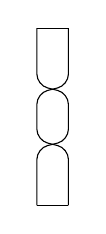
\begin{tikzpicture}[baseline]
				\node(xl1) at (-0.2,1){};
				\node(xr1) at (0.2,1){};	
				\node(xl2) at (-0.2, -1){};
				\node(xr2) at (0.2, -1){};
				\draw[rounded corners](xl1.north) to (-0.2,0.4) to (0.2, 0.3) to (0.2, -0.3) to (-0.2, -0.4) to (xl2.south);	
       				\draw[rounded corners](xr1.north) to (0.2,0.4) to (-0.2, 0.3) to (-0.2, -0.3) to (0.2, -0.4) to (xr2.south);
				\draw(xl1.north) to (xr1.north);
				\draw(xl2.south) to (xr2.south);	
			\end{tikzpicture} \\
			$b$ & & $t$ 
\end{tabular} \end{center}
% This operad $RB$ is also clearly an action operad, since we can just define $\pi^{RB}_n \colon RB_{n} \rightarrow \Sigma_n$ to act like $\pi^B_n$ on any braids, at which point the fact that $\pi(t) \in S_1 = \{e_1\}$ will automatically take care of the twists.

\begin{example}[(Action operad of cactus groups)]\label{ex:cactus-aop}
%\begin{enumerate}
%\item We now describe two less trivial action operads, those given by the braid groups (\cref{ex:braid_operad_B}), $\Lambda = B$, and the ribbon braid groups, $\Lambda = RB$. In each case, the homomorphism $\pi$ is given by taking underlying permutations, and the operad structure is given geometrically by using the procedure explained after \cref{broperad}. For $RB$, the fact that $\pi(t) \in \Sigma_1 = \{e_1\}$ automatically takes care of the twists. We refer the reader to \cite{fie-br} for more information about braided operads, and to \cite{sal-wahl, wahl-thesis} for information about the ribbon case.
The operad of $n$-fruit cactus groups defined by Henriques and Kamnitzer in \cite{hk-cobound} has an action operad structure that we will discuss in \cref{sec:exex-cactus}.
%\end{enumerate}
\end{example}

\begin{example}[(Action operad from an abelian group)]\label{ex:abgp-aop}
Every abelian group $A$ gives rise to an action operad $A^{\bullet}$ as follows. The group $A^{\bullet}(n)$ is the direct sum of $n$ copies of $A$, $A^{n}$. The identity element is required to be $e \in A^{1}$, and the multiplication is defined by
  \[
    \mu((a_{1}, \ldots, a_{n}); \underline{b_1}, \ldots, \underline{b_n}) = (a_{1}+\underline{b_{1}}, a_{2} + \underline{b_{2}}, \ldots, a_{n} + \underline{b_{n}})
  \]
where $\underline{b_{i}}$ is the string $b_{i1}, \ldots, b_{ik_{i}}$, and $a_{i} + \underline{b_{i}}$ is
  \[
    a_{i} + b_{i1}, a_{i} + b_{i2}, \ldots, a_{i} + b_{ik_{i}}.
  \]
The map $\pi_n \colon A^\bullet(n) \rightarrow \Sigma_n$ is the zero map. 
\end{example}

The characterisation of action operads in terms of maps $\pi$, $\beta$, and $\delta$ as in the above \cref{thm:charAOp} allows us to more easily check for counterexamples, as we show in the latter examples below. Some of these, such as the cyclic groups, reflexive groups, and hyperoctahedral groups, do however form crossed simplicial groups as described in \cref{rem:crossed}.

\begin{example}[(Non-examples: subgroups of symmetric groups)]\label{ex:counterex1}
By \cref{prop:surjortriv}, the only action operad $\pi \colon \Lambda \to \Sigma$ for which the homomorphisms $\pi_n$ are injective but not surjective is the action operad of trivial groups. 
Thus there is no family of proper, nontrivial subgroups of the symmetric groups that admits an action operad structure.
In particular, the families of cyclic groups $\{ C_n \}$, reflexive groups $\Lambda(n) = C_2$ of \cite{Kra87}, and alternating groups $\{ A_n \}$ do not admit action operad structures.
\end{example}

\begin{example}[(Non-example: hyperoctahedral groups)]\label{ex:counterex2}
Copied:

n Example 2.28 of \cite{zhang-grp}, Zhang describes one way in which the sequence of hyperoctahedral groups $H_n = C_2 \wr \Sigma_n$ do not form an action operad. We clarify that counterexample here, while also describing another. Elements of $H_n$ can be thought of as signed permutations or, equivalently, as $n \times n$ invertible matrices whose entries consist of $-1$, $0$, or $1$ and in which each row and column has exactly one non-zero entry. E.g., we can consider an element of $H_3$ as a permutation matrix and a $3$-tuple of elements of $C_2 = \{-1,1\}$, or simply as a signed permutation matrix:
  \[
    \left(\trans{2}{3}
    ;
    -1,1,-1\right)
    =
    \left(\begin{bmatrix}
    1 & 0 & 0 \\
    0 & 0 & 1 \\
    0 & 1 & 0
    \end{bmatrix}
    ;
    -1,1,-1\right)
    =
    \begin{bmatrix}
    -1 & 0 & 0 \\
    0 & 0 & -1 \\
    0 & 1 & 0
    \end{bmatrix}
    \in H_3.
  \]

In order to describe the hyperoctahedral groups as an action operad, we could use \cref{thm:charAOp} and define maps $\pi$, $\beta$, and $\delta$. The obvious map $\pi_n \colon H_n \rightarrow \Sigma_n$ takes the `absolute value' of a signed permutation matrix, giving back simply the underlying permutation. It seems obvious then to define $\beta$ to be the block sum of signed permutation matrices, in much the same way as for the symmetric groups. E.g.,
  \[
    \beta\left(
      \begin{bmatrix}
      -1 & 0 & 0 \\
      0 & 0 & -1 \\
      0 & 1 & 0
      \end{bmatrix},
      \begin{bmatrix}
      0 & 1 \\
      -1 & 0
      \end{bmatrix}
    \right)
    =
    \begin{bmatrix}
      -1 &  0 &  0 &  0 & 0 \\
      0  &  0 & -1 &  0 & 0 \\
      0  &  1 &  0 &  0 & 0 \\
      0  &  0 &  0 &  0 & 1 \\
      0  &  0 &  0 & -1 & 0
    \end{bmatrix}.
  \]
For the maps $\delta$, there seems to be two sensible options to try. The first captures Zhang's counterexample by first taking $r_n$ to be the order-reversing signed permutation matrix where all entries are $-1$, i.e., the $n \times n$ matrix with $-1$ in every entry of the anti-diagonal. Then we can define $\delta_{n;k_1,\ldots,k_n}(\sigma)$ to be the block sum $\beta(-r_{k_1},\ldots,-r_{k_n})$ acted on by the product of $r_n$ and $\sigma$. For example,
  \begin{align*}
    \delta_{3;2,1,3}\left(
    \begin{bmatrix}
      -1 & 0 & 0 \\
      0 & 0 & -1 \\
      0 & 1 & 0
      \end{bmatrix}
      \right)
      &=
      \left(
      r_3
      \begin{bmatrix}
      -1 & 0 & 0 \\
      0 & 0 & -1 \\
      0 & 1 & 0
      \end{bmatrix}
      \right)
      \ast
      \begin{bmatrix}
      -r_2 & 0 & 0 \\
      0 & -r_1 & 0 \\
      0 & 0 & -r_3
      \end{bmatrix}\\
&=
    \begin{bmatrix}
      0 & -1 & 0 \\
      0 & 0 & 1 \\
      1 & 0 & 0
      \end{bmatrix}
      \ast
      \begin{bmatrix}
      -r_2 & 0 & 0 \\
      0 & -r_1 & 0 \\
      0 & 0 & -r_3
      \end{bmatrix}\\
      &= \begin{bmatrix}
      0 & r_1 & 0\\
      0 & 0 & -r_3 \\
      -r_2 & 0 & 0
      \end{bmatrix}.
    \end{align*}
In particular, this gives $\delta_{1;n}([-1]) = r_n$ as in \cite{zhang-grp}. Taking $\sigma = (\trans{2}{3};-1,1,-1)$, as above, we can show that Axiom \ref{eq8} fails in \cref{thm:charAOp}. The left-hand side of the axiom would be
        \[
          \delta_{1;3}([-1])\beta(\sigma) = r_n \cdot \sigma =
          \begin{bmatrix}
          0 & -1 & 0 \\
          0 & 0 & 1 \\
          1 & 0 & 0
          \end{bmatrix}
        \]
However, the right-hand side of the axiom would be
  \[
    \beta(\sigma)\delta_{1;3}([-1]) = \sigma \cdot r_n =
    \begin{bmatrix}
    0 & 0 & 1 \\
    1 & 0 & 0 \\
    0 & -1 & 0
    \end{bmatrix}.
  \]
Clearly defining $\delta_{n;k_1,\ldots,k_n}(\sigma) = (\sigma \cdot r_n) \ast \beta(-r_{k_1},\ldots,-r_{k_n})$ would run into the same problem.

An alternative way of defining $\delta$ is to take $\delta_{n;k_1,\ldots,k_n}(\sigma) = \sigma \ast \beta(e_{k_1},\ldots,e_{k_n})$, without involving the order-reversing permutation $r_n$, having the effect of making $\delta_{1;n}([-1]) = -I_n$. This then does satisfy Axiom \ref{eq8}, but fails Axiom \ref{eq6} instead; working through the following counterexample shows this to be the case:
  \begin{align*}
    \delta_{3;2,1,3}\left(
    \begin{bmatrix}
    -1 & 0 & 0 \\
    0 & 0 & 1 \\
    0 & -1 & 0
    \end{bmatrix}
    \right)
    &\delta_{3;3,1,2}\left(
    \begin{bmatrix}
    0 & 0 & 1 \\
    0 & -1 & 0 \\
    -1 & 0 & 0
    \end{bmatrix}
    \right)\\
    &\neq
    \delta_{3;3,1,2}\left(
    \begin{bmatrix}
    -1 & 0 & 0 \\
    0 & 0 & 1 \\
    0 & -1 & 0
    \end{bmatrix}
    \begin{bmatrix}
    0 & 0 & 1 \\
    0 & -1 & 0 \\
    -1 & 0 & 0
    \end{bmatrix}
    \right).
  \end{align*}
\end{example}

%\begin{enumerate}
%\item Cyclic groups: In this case we would want to have $\Lambda(n) = C_n$, the cyclic group of order $n$, with $\pi_n$ being the underlying permutation. But these simply don't form an operad if we are to emulate the composition operation from the symmetric operad $\Sigma$. E.g., by denoting the generator of $C_n$ by $c_n$:
%  \begin{align*}
%    \mu(c_4 ; c_2, c_2) &= (1 \,\, 2 \,\, 3 \,\, 4)\trans{1}{2}\trans{3}{4} \\
%    &= \trans{1}{3} \\
%    &\neq c_4^n
%  \end{align*}
%for any $n \in \{1,2,3,4\}$.
%\item Reflexive groups \cite{Kra87}: Here we would like to take $\Lambda(n) = C_2 = \{e, c_2\}$ with $\pi_n(c_2)$ being the order-reversing permutation on $n$ elements. With these groups and the underlying permutations as described, we find that Axiom \ref{eq1} of \cref{thm:charAOp} is not satisfied. Either $\beta(c_2,c_2) = c_2$ or $\beta(c_2,c_2) = e$. Now
%  \[
%    \beta(\pi_2(c_2),\pi_2(c_2)) = \beta(\trans{1}{2},\trans{1}{2}) = \trans{1}{2}\trans{3}{4}.
%  \]
%But in the case that $\beta(c_2,c_2) = c_2$, then
%  \[
%    \pi_4(\beta(c_2,c_2)) = \pi_4(c_2) = \trans{1}{4}\trans{2}{3} \neq \trans{1}{2}\trans{3}{4}.
%  \]
%In the other case, then
%  \[
%    \pi_4(\beta(c_2,c_2)) = \pi_4(e) = e_4 \neq \trans{1}{2}\trans{3}{4}.
%  \]
%\item
% Hyperoctahedral groups: Can't remember what this fails to satisfy... Dan Graves came up with a counterexample, using the main action operad equivariance axiom, which was clearer than Zhang's description \cite{zhang-grp} - Example 2.28. Can show now that this is really saying that it fails Axiom \ref{eq8} of \cref{thm:charAOp} when taking $\delta_{1;n}(-1)$ to be the order-reversing permutation. If considering elements of the hyperoctahedral groups to be signed permutation matrices, then it may be the case that this works if taking $\delta_{1;n}(-1)$ to be the negative identity matrix.

% In Example 2.28 of \cite{zhang-grp}, Zhang describes how the sequence of hyperoctahedral groups $H_n = C_2 \wr \Sigma_n$ do not form an action operad, despite naturally being a crossed simplicial group. Thanks to Dan Graves, we can also describe directly which axioms of \cref{thm:charAOp} fail to be satisfied, clarifying Zhang's counterexample. On the one hand, if we take $\delta_{1;n}(-1)$ to be the order-reversing permutation, then this fails to satisfy Axiom \ref{eq8} of \cref{thm:charAOp}.

% QQQ Need to revisit this and remember how it works. Certain that it doesn't work for $\delta_{1;k}(\tau) = r_k$, but need to carefully check for when $\delta(\sigma)$ is a `permuted signed block identity' matrix(???).
%\item Alternating groups: If we take $\beta$ and $\delta$ to be analogues of the same maps for the symmetric groups, then we can easily produce non-even permutations using $\delta$: $\delta_{4;,0,0,1,1}(\trans{1}{2}\trans{3}{4})=\trans{1}{2} \notin A_2$ or $\delta_{4;1,1,1,2}(\trans{1}{2}\trans{3}{4}) = \trans{1}{2}\trans{3}{4}\trans{4}{5} \notin A_5$.
%\end{enumerate}
%\end{example}

\begin{rem}\label{rem:crossed}
The crossed simplicial groups of Krasauskas \cite{Kra87} and Fiedoriwicz and Loday \cite{FL91} are related to action operads in the following way. 
On objects, we define a functor $C \colon \mathbf{AOp} \rightarrow \mathbf{CSGrp}$ from the category of action operads to the category of crossed simplicial groups by defining $C(\Lambda)(n) = \Lambda(n+1)$. 
The face and degeneracy maps of the underlying simplicial structure are defined using the operadic composition of $\Lambda$ as in \cite[Construction~1.1]{Kra96} or \cite[Section~2]{ber-simplicial}. 
On morphisms, something\ngnote{is it just $C(f)(n) = f_{n+1}$? That seems conservative to me}.
This functor is neither faithful nor conservative.
\end{rem}
%Salvatore-Wahl:  Framed disks operads\ldots
% \begin{nota}\label{beta_to_oplus}
% Leaning more heavily into the interpretation that the operations denoted $\beta$ above are block sums, we also write $g_1 \oplus g_2 \oplus \cdots \oplus g_n$ for
% $\beta(g_1, g_2, \ldots, g_n)$.
% \end{nota}




\section{Action Operads as Extensions}

In this short section, we situate action operads between operads in the category of groups and symmetric operads.
We prove two main results.
In \cref{prop:Z}, we prove that operads in the category of groups are precisely the same as action operads for which the homomorphisms $\pi_n$ are all the zero map; these are called ``non-crossed group operads'' in \cite{zhang-grp}.
We then turn to studying kernels, images, and short exact sequences of action operads.
We finally prove, in \cref{cor:extension}, that every action operad with surjective $\pi_n$'s can be expressed as an extension of the action operad $\Sigma$ by an operad in the category of groups.

\begin{rem}[(Operads in the category of groups)]\label{rem:op-in-grp}
The category $\mb{Grp}$ of groups and group homomorphisms is symmetric monoidal using the cartesian product of groups.
Thus we can form the category of operads in the category of groups, denoted $\mb{Op}(\mb{Grp})$, as in \cref{rem:V-and-coll}.
The objects of this category are operads $P$ in $\mb{Sets}$ with the additional data of a group structure on each $P(n)$ such that operadic multiplication is a group homomorphism and $\id = e_1$ in $P(1)$; morphisms $f \colon P \to Q$ are those maps of operads such that $f_n \colon P(n) \to Q(n)$ is a group homomorphism for each $n$.
\end{rem}

\begin{prop}\label{prop:Z-obj}
Let $P$ be an operad in $\mb{Grp}$. Then there is an action operad, denoted $Z(P)$, with
\begin{itemize}
\item $Z(P)(n) = P(n)$,
\item the same operadic multiplication as $P$, and
\item each $\pi_n \colon P(n) \to \Sigma_n$ the zero map.
\end{itemize}
Furthermore, if $\Lambda$ is an action operad for which each $\pi_n$ is the zero map, then the groups $\Lambda(n)$ define an operad in $\mb{Grp}$ using the operadic multiplication of $\Lambda$.
\end{prop}
\begin{proof}
It is easy to verify, using \cref{eqn:ao_axiom} of \cref{Defi:aop}, that the operadic multiplication $\mu$ of an action operad is a group homomorphism if and only if $\pi_{n}$ is zero for all $n$.
\end{proof}

\begin{prop}\label{prop:Z}
The assignment on objects $P \mapsto Z(P)$ extends to a functor 
\[
Z \colon  \mb{Op}(\mb{Grp}) \rightarrow \mb{AOp}.
\]
This functor is full, faithful, and its image at the level of objects is precisely the collection of action operads $\Lambda$ for which each $\pi_n$ is the zero map.
\end{prop}
\begin{proof}
Let $f \colon P \to Q$ be a morphism in $\mb{Op}(\mb{Grp})$, meaning that $f$ consists of a family of group homomorphisms $f_n \colon P(n) \to Q(n)$ that define a map of operads.
Define $Z(f)_n = f_n$. We must check that these functions define a map of action operads; functoriality will follow immediately, as composition and identities in both $\mb{Op}(\mb{Grp})$ and $\mb{AOp}$ are given levelwise.
Since each action operad $Z(P)$ has $\pi_n$ the zero map for all $n$, the first numbered axiom in \cref{Defi:mapaop} is satisfied trivially.
The second numbered axiom follows from the definition of a morphism in $\mb{Op}(\mb{Grp})$.
This completes the proof that $Z(f)$ is a map of action operads, and the same reasoning shows that every map of action operads $g \colon Z(P) \to Z(Q)$ is $Z(g')$ for a unique $g' \colon P \to Q$ in $\mb{Op}(\mb{Grp})$, thus $Z$ is full and faithful.
\end{proof}

\begin{prop}\label{prop:im-and-ker-aop}
Let $f \colon \Lambda \to \Lambda'$ be a map of action operads.
\begin{enumerate}
\item The groups
  \[
    \mathrm{Ker}\,f_n = \{x \in \Lambda(n)~\colon~f(x) = e_{n} \}
  \]
form an action operad for which the inclusion $\mathrm{Ker}\,f \hookrightarrow \Lambda$ is a map of action operads.
\item The groups
  \[
    \mathrm{Im}\,f_n = \{f(x)~\colon~x \in \Lambda(n)\}
  \]
form an action operad for which the inclusion $\mathrm{Im}\,\pi \hookrightarrow \Lambda'$ is a map of action operads.
\end{enumerate}
\end{prop}
\begin{proof}
For the first part, we start by defining $\pi_n^{\mathrm{Ker}\,f} \colon \mathrm{Ker}\,f_n \to \Sigma_n$ as the composite group homomorphism
\[
\mathrm{Ker}\,f_n \hookrightarrow \Lambda(n) \stackrel{\pi_n^{\Lambda}}{\to} \Sigma_n.
\]
Since $\pi^{\Lambda} = \pi^{\Lambda'} \circ f$, the composites $\pi_n^{\mathrm{Ker}\,f}$ are all the zero map.
Next we verify that the subgroups $\mathrm{Ker}\,f_n$ are closed under operadic multiplication. 
Let $y \in \mathrm{Ker}\,f_n$ and $x_i \in \mathrm{Ker}\,f_{k_i}$ for $i=1, \ldots, n$.
Then
\begin{align*}
f \big( \mu(y; x_1, \ldots, x_n) \big) & = \mu\big( f(y); f(x_1), \ldots, f(x_n) \big) \\
& = \mu(e_n; e_{k_1}, \ldots, e_{k_n} ) \\ 
& = e_{k_1 + \cdots + k_n}
\end{align*}
by the assumption that $f$ is a map of operads, that $y$ and each $x_i$ is in the kernel, and \cref{lem:calclem}, showing that the kernel subgroups are closed under operadic multiplication.
The operadic identity $\id \in \Lambda(1)$ is an element of $\mathrm{Ker}\,f_1$ because it is equal to $e_1$ by \cref{lem:calclem}.
Thus the groups $\mathrm{Ker}\,f_n$ form a sub-operad of $\Lambda$, and the action operad axiom \cref{eqn:ao_axiom} of \cref{Defi:aop} for $\mathrm{Ker}\,f$ follows immediately from the same axiom for $\Lambda$.
This completes the proof of the first claim, and in fact shows, via \cref{prop:Z-obj}, that these groups constitute an operad in $\mb{Grp}$.

For the second part, we start by defining $\pi_n^{\mathrm{Im}\,f} \colon \mathrm{Im}\,f_n \to \Sigma_n$ as the composite group homomorphism
\[
\mathrm{Im}\,f_n \hookrightarrow \Lambda'(n) \stackrel{\pi_n^{\Lambda'}}{\to} \Sigma_n.
\]
These subgroups are closed under operadic multiplication in $\Lambda'$ using that $f$ is a map of action operads.
The operadic identity $\id \in \Lambda'(1)$ is an element of $\mathrm{Im}\,f_1$ because it is equal to $e_1$ by \cref{lem:calclem}.
This completes the proof that the groups $\mathrm{Im}\,f_n$ form a sub-operad of $\Lambda'$, and the action operad axiom \cref{eqn:ao_axiom} of \cref{Defi:aop} for $\mathrm{Im}\,f$ follows immediately from the same axiom for $\Lambda'$, finishing the proof of the second claim.
\end{proof}

\begin{example}[(Action operads of pure braids, pure ribbon braids)]\label{ex:pure-braids}
%Thus we see that an action operad is either an operad in groups, or is an extension of $\Sigma$ by an operad in groups. 
The $n$th pure braid group, $PB_n$, is defined as the kernel of the homomorphism $\pi_n \colon B_n \to \Sigma_n$, or equivalently as the subgroup of the $n$th braid group consisting of those braids with underlying permutation the identity.
\cref{prop:im-and-ker-aop} gives a simple proof that the pure braid groups form an operad in the category of groups.
Similarly, the pure ribbon braid group, $PRB_n$, is defined as the kernel of $\pi_n \colon RB_n \to \Sigma_n$, and these groups also constitute an operad in the category of groups.

\end{example}

\begin{rem}[(Kernels and images of $\pi$)]\label{rem:im-and-ker-Sigma}
We note that if $(\Lambda, \pi)$ is an action operad, then we can apply the results of \cref{prop:im-and-ker-aop} to $\pi$ by \cref{prop:pi-in-aop}.
The action operad $\mathrm{Ker}\,\pi_n$ will then be an operad in groups, and the action operad $\mathrm{Im}\,\pi_n$ will be a sub-action operad of $\Sigma$.
By \cref{prop:surjortriv}, this means that the action operad $\mathrm{Im}\,\pi_n$ is either $\Sigma$ or the trivial action operad $T$ (\cref{example:aop-triv}).
\end{rem}

%We have the following corollary.
%\begin{cor}\label{corZ}
%For an action operad $\Lambda$, the sets
%  \[
%    \mathrm{Ker}\,\pi_n = \{g \in \Lambda(n)~\colon~\pi_{n}(g) = e_{n} \}
%  \]
%form an action operad for which the inclusion $\mathrm{Ker}\,\pi \hookrightarrow \Lambda$ is a map of action operads.
%\end{cor}
%\begin{proof}
%For $\textrm{Ker}\,\pi \hookrightarrow \Lambda$ to be a map of action operads, we must define the map $\textrm{Ker}\,\pi \rightarrow \Sigma$ to be zero,  and we must check that the operadic multiplication of elements in the kernel is also in the kernel. This last fact is a trivial consequence of $\pi$ being an operad map.
%\end{proof}
%
%\begin{cor}\label{image}
%For an action operad $\Lambda$, the sets
%  \[
%    \mathrm{Im}\,\pi_n = \{\pi_n(g)~\colon~g \in \Lambda(n)\}
%  \]
%form an action operad for which the inclusion $\mathrm{Im}\,\pi \hookrightarrow \Sigma$ is a map of action operads.
%\end{cor}
%\begin{proof}
%The operad multiplication of elements in the image is also in the image, as is the unit element in $\mathrm{Im}\,\pi_1$, following again as a consequence of $\pi$ being an operad map. The map $\mathrm{Im}\,\pi \hookrightarrow \Sigma$ is an inclusion and so is immediately seen to be a map of action operads.
%\end{proof}

\begin{Defi}\label{Defi:ses-aop}
A \emph{short exact sequence of action operads} consists of action operads $\Lambda_1, \Lambda_2, \Lambda_3$ and maps of action operads $f \colon \Lambda_1 \to \Lambda_2$, $g \colon \Lambda_2 \to \Lambda_3$ such that
\begin{itemize}
\item the action operad $\mathrm{Ker}\,f$ is the trivial action operad $T$,
\item the action operad $\mathrm{Im}\,f$ is the action operad $\mathrm{Ker}\,g$, and
\item the action operad $\mathrm{Im}\,g$ is the action operad $\Lambda_3$.
\end{itemize}
We denote such a short exact sequence as
\[
T \to \Lambda_1 \stackrel{f}{\to} \Lambda_2 \stackrel{g}{\to} \Lambda_3 \to T,
\]
and we say that a short exact sequence exhibits \emph{$\Lambda_2$ as an extension of $\Lambda_3$ by $\Lambda_1$}.
\end{Defi}

The following corollary puts \cref{rem:im-and-ker-Sigma} into the language of short exact sequences and extensions.

\begin{cor}\label{cor:extension}
Let $(\Lambda, \pi)$ be an action operad and assume that every homomorphism $\pi_n \colon \Lambda(n) \to \Sigma_n$ is surjective.
Then there is a short exact sequence of action operads
%Every action operad $\Lambda$ with nontrivial $\pi$ fits into a short exact sequence
  \[
    T \rightarrow \mathrm{Ker}\,\pi \hookrightarrow \Lambda \stackrel{\pi}{\longrightarrow} \Sigma \rightarrow T.
  \]
%by which we mean this is a sequence of action operad maps which is an exact sequence of groups at each $n$.
\end{cor}

\section{Presentations for Action Operads}

A useful method for constructing new examples of some given algebraic structure is through the use of presentations. A presentation consists of generating data together with relations between generators using the operations of the algebra involved. In categorical terms, the generators and relations are both given as free gadgets on some underlying data, and the presentation itself is a coequalizer. This section will establish the categorical structure necessary to give presentations for action operads, and then explain how such a presentation is reflected in the associated club and $2$-monad. The most direct route to the desired results uses the theory of locally finitely presentable categories. We recall the main definitions briefly, but refer the reader to \cite{ar} for additional details.

\begin{Defi}\label{def:filtered}
  A \textit{filtered category} is a nonempty category $C$ such that
    \begin{itemize}
      \item if $a,b$ are objects of $C$, then there exists another object $c \in C$ and morphisms $a \rightarrow c, b \rightarrow c$; and
      \item if $f,g \colon a \rightarrow b$ are parallel morphisms in $C$, then there exists a morphism $h \colon b \rightarrow c$ such that $hf = hg$.
    \end{itemize}
\end{Defi}

\begin{Defi}
  A \emph{filtered colimit} is a colimit over a filtered category.
\end{Defi}

\begin{Defi}
  Let $C$ be a category with all filtered colimits. An object $x \in C$ is \textit{finitely presentable} if the representable functor $C(x, -) \colon C \rightarrow \mb{Sets}$ preserves filtered colimits.
\end{Defi}

\begin{Defi}
  A \textit{locally finitely presentable category} is a category $C$ such that
  \begin{itemize}
    \item $C$ is cocomplete and
    \item there exists a small subcategory $C_{fp} \subseteq C$ of finitely presentable objects such that any object $x \in C$ is the filtered colimit of some diagram in $C_{fp}$.
  \end{itemize}
\end{Defi}

The definition of a locally finitely presentable category has many equivalent variants, but we find this one most practicable to work with in this setting.

\begin{thm}
The category $\mb{AOp}$ is locally finitely presentable.
\end{thm}
\begin{proof}
First note that we can define a category $\mb{Op}^{g}$, whose objects are operads $P$ in which each $P(n)$ also carries a group structure. This is an equational theory using equations with only finitely many elements, so $\mb{Op}^{g}$ is locally finitely presentable \cite[Corollary 3.7]{ar}. A slice category of a locally finitely presentable category is itself locally finite presentable \cite[Proposition 1.57]{ar} and since the symmetric operad is an object of $\mb{Op}^{g}$, the slice category $\mb{Op}^{g}/\Sigma$ is locally finitely presentable.

There is an obvious inclusion functor $\mb{AOp} \hookrightarrow \mb{Op}^{g}/\Sigma$. Now $\mb{AOp}$ is a full subcategory of $\mb{Op}^{g}/\Sigma$ which is closed under products, subobjects. Since any object of $\mb{Op}^{g}/\Sigma$ isomorphic to an action operad is in fact an action operad, the inclusion   $\mb{AOp} \hookrightarrow \mb{Op}^{g}/\Sigma$ is actually the inclusion of a reflective subcategory. One can easily check that $\mb{AOp}$ is in fact closed under all limits and filtered colimits in $\mb{Op}^{g}/\Sigma$, so by the Reflection Theorem (2.48 in \cite{ar}), $\mb{AOp}$ is locally finitely presentable.
\end{proof}

\begin{Defi}
  Let $\SS$ be the set which is the disjoint union of the underlying sets of all the symmetric groups. Then $\mb{Sets}/\SS$ is the slice category over $\SS$ with objects $(X,f)$ where $X$ is a set and $f \colon X \rightarrow \SS$ and morphisms $(X_{1}, f_{1}) \rightarrow (X_{2}, f_{2})$ are those functions $g \colon X_{1} \rightarrow X_{2}$ such that $f_{1} = f_{2}g$. We call an object $(X,f)$ a \textit{collection over $\SS$}.
\end{Defi}

\begin{rem}
In standard presentations of the theory of operads (see, for example, \cite{mss-op}), a nonsymmetric operad will have an underlying collection (or $\mathbb{N}$-indexed collection of sets) while a symmetric operad will have an underlying symmetric collection (or $\mathbb{N}$-indexed collection of sets in which the $n$th set has an action of $\Sigma_{n}$). Our collections over $\SS$ more closely resemble the former as there is no group action present.
\end{rem}

\begin{example}
One can easily form new action operads from old ones by taking limits. To take a limit of a diagram in $\mb{AOp}$, one forgets down to the category of operads over $\Sigma$ and takes the limit there. Concretely, products in $\mb{AOp}$ are computed as products in $\mb{Op}/\Sigma$ which themselves are (possibly wide) pullbacks in the category of operads. This pullback will then be computed levelwise, showing that at each dimension there is a group structure with a group homomorphism to the appropriate $\Sigma_{n}$ and that the final action operad axiom holds since it does in each component. The equalizer of a pair of maps will then just be the levelwise equalizer. This shows that the pointwise product of an action operad $P$ with an action operad of the form $Z(Q)$ (as in \cref{Z}) is again an action operad, but the pointwise product of two arbitrary action operads might not be.
\end{example}
\begin{thm}\label{underlyingSS}
There exists a forgetful functor $U \colon \mb{AOp} \rightarrow \mb{Sets}/\SS$ which preserves all limits and filtered colimits.
\end{thm}

\begin{proof}
For a given action operad $\Lambda$, we put $U(\Lambda) = \left(\coprod_{\mathbb{N}} \Lambda(n), \coprod_{\mathbb{N}} \pi_n \right)$ and this easily extends to a mapping on morphisms using the universal property of the coproduct. The preservation of filtered colimits follows from the fact that these are computed pointwise, together with the fact that every map between action operads preserves underlying permutations.
As equalizers are computed levelwise, and the product $\Lambda \times \Lambda'$ has underlying operad the pullback $\Lambda \times_{\Sigma} \Lambda'$; this pullback is itself computed levelwise. Together, these imply that $U$ also preserves all limits.
\end{proof}

\begin{cor}
$U$ has a left adjoint $F \colon \mb{Sets}/\SS \rightarrow \mb{AOp}$, the free action operad functor.
\end{cor}
\begin{proof}
The category $\mb{Sets}/\SS$ is locally finitely presentable as it is equivalent to the functor category $[\SS, \mb{Sets}]$ (here $\SS$ is treated as a discrete category) and any presheaf category is locally finitely presentable. The functor $U$ preserves limits and filtered colimits between locally finitely presentable categories, so has a left adjoint (see Theorem 1.66 in \cite{ar}).
\end{proof}

\begin{Defi}
  A \textit{presentation} for an action operad $\Lambda$ consists of
  \begin{itemize}
    \item a pair of collections over $\SS$ denoted $\mathbf{g}, \mathbf{r}$,
    \item a pair of maps $s_{1}, s_{2} \colon F\mathbf{r} \rightarrow F\mathbf{g}$ between the associated free action operads, and
    \item a map $p \colon F\mathbf{g} \rightarrow \Lambda$ of action operads exhibiting $\Lambda$ as the coequalizer of $s_{1},s_{2}$.
  \end{itemize}
\end{Defi}

\section{Action Operads as Clubs}

Kelly's theory of clubs \cite{kelly_club1, kelly_club0, kelly_club2} was designed to simplify and explain certain aspects of coherence results, namely the fact that many coherence results rely on extrapolating information about general free objects for a $2$-monad $T$ from information about the specific free object $T1$ where $1$ denotes the terminal category. This occurs, for example, in the study of the many different flavors of monoidal category:  plain monoidal category, braided monoidal category, symmetric monoidal category, and so on. This section will explain how every action operad gives rise to a club, as well as compute the clubs which arise as the image of this procedure.

We begin by reminding the reader of the notion of a club, or more specifically what Kelly \cite{kelly_club1,kelly_club2} calls a club over $\mb{P}$. We will only be interested in clubs over $\mb{P}$, and thusly shorten the terminology to club from this point onward. Defining clubs is accomplished most succinctly using Leinster's terminology of generalized operads \cite{leinster}.

\begin{Defi}
Let $C$ be a category with finite limits.
\begin{enumerate}
\item A monad $T \colon C \rightarrow C$ is \textit{cartesian} if the functor $T$ preserves pullbacks, and the naturality squares for the unit $\eta$ and the multiplication $\mu$ for $T$ are all pullbacks.
\item The category of \textit{$T$-collections}, $T\mbox{-}\mb{Coll}$, is the slice category $C/T1$, where $1$ denotes the terminal object.
\item Given a pair of $T$-collections $X \stackrel{x}{\rightarrow} T1, Y \stackrel{y}{\rightarrow} T1$, their \textit{composition product} $X \circ Y$ is given by the pullback below together with the morphism along the top.
  \[
    \xy
      (0,0)*+{X \circ Y} ="00";
      (15,0)*+{TY} ="10";
      (30,0)*+{T^{2}1} ="20";
      (45,0)*+{T1} ="30";
      (0,-10)*+{X} ="01";
      (15,-10)*+{T1} ="11";
      {\ar^{} "00" ; "10"};
      {\ar^{Ty} "10" ; "20"};
      {\ar^{\mu} "20" ; "30"};
      {\ar^{T!} "10" ; "11"};
      {\ar_{x} "01" ; "11"};
      {\ar^{} "00" ; "01"};
      (3,-3)*{\lrcorner};
    \endxy
  \]
\item The composition product, along with the unit of the adjunction $\eta \colon 1 \rightarrow T1$, give $T\mbox{-}\mb{Coll}$ a monoidal structure. A \textit{$T$-operad} is a monoid in $T\mbox{-}\mb{Coll}$.
\end{enumerate}
\end{Defi}

\begin{rem}
Everything in the above definition can be $\mb{Cat}$-enriched without any substantial modifications. Thus we require our ground $2$-category to have finite limits in the enriched sense, and the slice and pullbacks are the $2$-categorical (and not bicategorical) versions. If we take this $2$-category to be $\mb{Cat}$, then in each case the underlying category of the $2$-categorical construction is given by the corresponding $1$-categorical version. From this point, we will not distinguish between the $1$-dimensional and $2$-dimensional theory. Our interest, of course, is in the $2$-dimensional version.
\end{rem}

Let $\Sigma$ be the operad of symmetric groups. This is the terminal object of the category of action operads, with each $\pi_{n}$ the identity map. Then $\underline{E\Sigma}$ is a $2$-monad on $\mb{Cat}$, and by results in \cref{sec:propofopsincat} it is cartesian.

\begin{Defi}
A \textit{club} is a $T$-operad in $\mb{Cat}$ for $T = \underline{E\Sigma}$.
\end{Defi}

\begin{rem}
The category $\mb{P}$ in Kelly's terminology is the result of applying $\underline{E\Sigma}$ to $1$, and can be identified with $B\Sigma = \coprod B\Sigma_{n}$.
\end{rem}

It is useful to break down the definition of a club. A club consists of
\begin{enumerate}
\item a category $K$ together with a functor $K \rightarrow B \Sigma$,
\item a multiplication map $K \circ K \rightarrow K$, and
\item a unit map $1 \rightarrow K$
\end{enumerate}
satisfying the axioms to be a monoid in the monoidal category of $E\Sigma$-collections. By the definition of $K \circ K$ as a pullback, objects are tuples of objects of $K$ $(x; y_{1}, \ldots, y_{n})$ where $\pi(x) = n$. A morphism
  \[
    (x; y_{1}, \ldots, y_{n}) \rightarrow (z; w_{1}, \ldots, w_{m})
  \]
exists only when $n=m$ (since $B\Sigma$ only has endomorphisms) and then consists of a morphism $f \colon x \rightarrow z$ in $K$ together with morphisms $g_{i} \colon y_{i} \rightarrow z_{\pi(x)(i)}$ in $K$.

\begin{nota}\label{nota:clubmult}
For a club $K$ and a morphism $(f; g_{1}, \ldots, g_{n})$ in $K \circ K$, we write $f(g_{1}, \ldots, g_{n})$ for the image of the morphism under the functor $K \circ K \rightarrow K$.
\end{nota}

We will usually just refer to a club by its underlying category $K$.


\begin{thm}
Let $\Lambda$ be an action operad. Then the map of operads $\pi \colon \Lambda \rightarrow \Sigma$ gives the category $B\Lambda = \coprod B\Lambda(n)$ the structure of a club.
\end{thm}
\begin{proof}
To give the functor $B\pi \colon B\Lambda \rightarrow B \Sigma$ the structure of a club it suffices (see \cite{leinster}) to show that
\begin{itemize}
\item the induced monad, which we will show to be $\underline{E\Lambda}$, is a cartesian monad on $\mb{Cat}$,
\item the transformation $\tilde{\pi} \colon \underline{E\Lambda} \Rightarrow \underline{E\Sigma}$ induced by the functor $E\pi$ is cartesian, and
\item $\tilde{\pi}$ commutes with the monad structures.
\end{itemize}
The monad $\underline{E\Lambda}$ is always cartesian by results of \cref{sec:propofopsincat}. The transformation $\tilde{\pi}$ is the coproduct of the maps $\tilde{\pi}_{n}$ which are induced by the universal property of the coequalizer as shown below.
  \[
    \xy
      (0,0)*+{\scriptstyle E\Lambda(n) \times \Lambda(n) \times X^n} ="00";
      (0,-15)*+{\scriptstyle E\Sigma_{n} \times \Sigma_{n} \times X^n} ="01";
      (30,0)*+{\scriptstyle E\Lambda(n) \times X^n} ="10";
      (30,-15)*+{\scriptstyle E\Sigma_{n} \times X^n} ="11";
      (60,0)*+{\scriptstyle E\Lambda(n) \times_{\Lambda(n)} X^n} ="20";
      (60,-15)*+{\scriptstyle E\Sigma_{n} \times_{\Sigma_{n}}  X^n} ="21";
      {\ar (11,1)*{}; (22,1)*{} };
      {\ar (11,-1)*{}; (22,-1)*{} };
      {\ar_{E\pi \times \pi \times 1} "00" ; "01"};
      {\ar (10,-14)*{}; (23,-14)*{} };
      {\ar (10,-16)*{}; (23,-16)*{} };
      {\ar_{E\pi \times 1} "10" ; "11"};
      {\ar@{.>}^{\tilde{\pi}_{n}} "20" ; "21"};
      {\ar "10" ; "20"};
      {\ar "11" ; "21"};
    \endxy
  \]
Naturality is immediate, and since $\pi$ is a map of operads $\tilde{\pi}$ also commutes with the monad structures.

It only remains to show that $\tilde{\pi}$ is cartesian and that the induced monad is actually $\underline{E\Lambda}$. Since the monads $\underline{E\Lambda}$ and $\underline{E\Sigma}$ both decompose into a disjoint union of functors, we only have to show that, for any $n$, the square below is a pullback.
  \[
    \xy
      (0,0)*+{\coeq{E\Lambda}{X}{\Lambda}{n}} ="00";
      (0,-10)*+{B\Lambda(n)} ="01";
      (35,0)*+{E\Sigma_{n} \times_{\Sigma_{n}} X^n} ="10";
      (35,-10)*+{B\Sigma_{n}} ="11";
      {\ar^{} "00" ; "10"};
      {\ar^{} "10" ; "11"};
      {\ar^{} "00" ; "01"};
      {\ar^{} "01" ; "11"};
    \endxy
  \]
By \cref{coeq-lem}
%(QQQ happy with this reference? QQQ Seems like the right thing?)
, this amounts to showing that the square below is a pullback.
  \[
    \xy
      (0,0)*+{\left(E\Lambda(n) \times X^n\right)/\Lambda(n)} ="00";
      (0,-10)*+{B\Lambda(n)} ="01";
      (35,0)*+{\left(E\Sigma_{n} \times X^n\right)/\Sigma_{n}} ="10";
      (35,-10)*+{B\Sigma_{n}} ="11";
      {\ar^{} "00" ; "10"};
      {\ar^{} "10" ; "11"};
      {\ar^{} "00" ; "01"};
      {\ar^{} "01" ; "11"};
    \endxy
  \]
Here, $(A \times B)/G$ is the category whose objects are equivalence classes of pairs $(a,b)$ where $(a,b) \sim (ag, g^{-1}b)$, and similarly for morphisms. Now the bottom map is clearly bijective on objects since these categories only have one object. An object in the top right is an equivalence class
  \[
    [\sigma; x_{1}, \ldots, x_{n}] = \left[e; x_{\sigma^{-1}(1)}, \ldots, x_{\sigma^{-1}(n)}\right].
  \]
A similar description holds for objects in the top left, with $g \in \Lambda(n)$ replacing $\sigma$ and $\pi(g)^{-1}$ replacing $\sigma^{-1}$ in the subscripts. The map along the top sends $[g; x_{1}, \ldots, x_{n}]$ to $[\pi(g); x_{1}, \ldots, x_{n}]$, and thus sends $[e; x_{1}, \ldots, x_{n}]$ to $[e; x_{1}, \ldots, x_{n}]$, giving a bijection on objects.

Now a morphism in $(E\Lambda(n) \times X^{n})/\Lambda(n)$ can be given as
  \[
    [e; x_{1}, \ldots, x_{n}] \stackrel{[!; f_{i}]}{\longrightarrow} [g; y_{1}, \ldots, y_{n}].
  \]
Mapping down to $B\Lambda(n)$ gives $ge^{-1} = g$, while mapping over to $(E\Sigma_{n} \times X^{n})/\Sigma_{n}$ gives $[!; f_{i}]$ where $! \colon e \rightarrow \pi(g)$ is now a morphism in $E\Sigma_{n}$. In other words, a morphism in the upper left corner of our putative pullback square is determined completely by its images along the top and lefthand functors. Furthermore, given $g \in \Lambda(n)$, $\tau = \pi(g)$, and morphisms $f_{i} \colon x_{i} \rightarrow y_{i}$ in $X$, the morphism $[! \colon e \rightarrow g; f_{i}]$ maps to the pair $(g, [! \colon e \rightarrow \tau; f_{i}])$, completing the proof that this square is indeed a pullback.
\end{proof}

The club, which we now denote $K_{\Lambda}$, associated to $E\Lambda$ has the following properties. First, the functor $K_{\Lambda} \rightarrow B\Sigma$ is a functor between groupoids. Second, the functor $K_{\Lambda} \rightarrow B\Sigma$ is  bijective-on-objects. We claim that these properties characterize those clubs which arise from action operads. Thus the clubs arising from action operads are very similar to PROPs \cite{mac_prop, markl_prop}.

\begin{thm}\label{thm:club=operad}
Let $K$ be a club such that
\begin{itemize}
\item the map $K \rightarrow B\Sigma$ is bijective on objects and
\item $K$ is a groupoid.
\end{itemize}
Then $K \cong K_{\Lambda}$ for some action operad $\Lambda$. The assignment $\Lambda \mapsto K_{\Lambda}$ is a full and faithful embedding of the category of action operads $\mb{AOp}$ into the category of clubs.
\end{thm}
\begin{proof}
Let $K$ be such a club. Our hypotheses immediately imply that $K$ is a groupoid with objects in bijection with the natural numbers; we will now assume the functor $K \rightarrow B\Sigma$ is the identity on objects. Let $\Lambda(n) = K(n,n)$. Now $K$ comes equipped with a functor to $B\Sigma$, in other words group homomorphisms $\pi_{n} \colon \Lambda(n) \rightarrow \Sigma_{n}$. We claim that the club structure on $K$ makes the collection of groups $\{ \Lambda(n) \}$ an action operad. In order to do so, we will employ \cref{thm:charAOp}.

First, we give the group homomorphism $\beta$ using \cref{nota:clubmult}. Define
  \[
    \beta(g_{1}, \ldots, g_{n}) = e_{n}(g_{1}, \ldots, g_{n})
  \]
 (see \ref{nota:clubmult}) where $e_{n}$ is the identity morphism $n \rightarrow n$ in $K(n,n)$. Functoriality of the club multiplication map immediately implies that this is a group homomorphism. Second, we define the function $\delta$ in a similar fashion:
  \[
    \delta_{n; k_{1}, \ldots, k_{n}}(f) = f(e_{1}, \ldots, e_{n}),
  \]
where here $e_{i}$ is the identity morphism of $k_{i}$ in $K$.

There are now nine axioms to verify in \cref{thm:charAOp}. The club multiplication functor is a map of collections, so a map over $B\Sigma$; this fact immediately implies that Axioms \eqref{eq1} (using morphisms in $K \circ K$ with only $g_{i}$ parts) and \eqref{eq4} (using morphisms in $K \circ K$ with only $f$ parts) hold. The mere fact that multiplication is a functor also implies Axioms \eqref{eq6} (once again using morphisms with only $f$ parts) and \eqref{eq8} (by considering the composite of a morphism with only an $f$ with a morphism with only $g_{i}$'s). Axiom \eqref{eq2} is the equation $e_{1}(g) = g$ which is a direct consequence of the unit axiom for the club $K$; the same is true of Axiom \eqref{eq5}. Axioms \eqref{eq3}, \eqref{eq7},  and \eqref{eq9} all follow from the associativity of the club multiplication.

Finally, we would like to show that this gives a full and faithful embedding
    \[
        K_{-} \colon \mb{AOp} \rightarrow \mb{Club}
    \]
of the category of action operads into the category of clubs. Let $f, f' \colon \Lambda \rightarrow \Lambda'$ be maps between action operads. Then if $K_{f} = K_{f'}$ as maps between clubs, then they must be equal as functors $K_{\Lambda} \rightarrow K_{\Lambda'}$. But these functors are nothing more than the coproducts of the functors
  \[
    B(f_{n}), B(f_{n}') \colon B\Lambda(n) \rightarrow B\Lambda'(n),
  \]
and the functor $B$ from groups to categories is faithful, so $K_{-}$ is also faithful. Now let $f \colon K_{\Lambda} \rightarrow K_{\Lambda'}$ be a maps of clubs. We clearly get group homomorphisms $f_{n} \colon \Lambda(n) \rightarrow \Lambda'(n)$ such that $\pi^{\Lambda}_{n} = \pi^{\Lambda'}_{n} f_{n}$, so we must only show that the $f_{n}$ also constitute an operad map. Using the description of the club structure above in terms of the maps $\beta, \delta$, we are able to see that commuting with the club multiplication implies commuting with both of these, which in turn is equivalent to commuting with operad multiplication. Thus $K_{-}$ is full as well.
\end{proof}

\begin{rem}
First, one should note that being a club over $B\Sigma$ means that every $K$-algebra has an underlying strict monoidal structure. Second, requiring that $K \rightarrow B\Sigma$ be bijective on objects ensures that $K$ does not have  operations other than $\otimes$, such as duals or internal hom-objects, from which to build new types of objects. Finally, $K$ being a groupoid ensures that all of the ``constraint morphisms'' that exist in algebras for $K$ are invertible.

These hypotheses could be relaxed somewhat. Instead of having a club over $B\Sigma$, we could have a club over the free symmetric monoidal category on one object (note that the free symmetric monoidal category monad on $\mb{Cat}$ is still cartesian). This would produce $K$-algebras with underlying monoidal structures which are not necessarily strict. This change should have relatively little impact on how the theory is developed. Changing $K$ to be a category instead of a groupoid would likely have a larger impact, as the resulting action operads would have monoids instead of groups at each level. We have made repeated use of inverses throughout the proofs in the basic theory of action operads, and these would have to be revisited if groups were replaced by monoids in the definition of action operads.
\end{rem}

In \cite{kelly_club1}, Kelly discusses clubs given by generators and relations. His generators include functorial operations more general than what we are interested in here, and the natural transformations are not required to be invertible. In our case, the only generating operations we require are those of a unit and tensor product, as the algebras for $E\Lambda$ are always strict monoidal categories with additional structure. Tracing through his discussion of generators and relations for a club gives the following theorem.

\begin{thm}\label{pres1}
Let $\Lambda$ be an action operad with presentation given by $(\mathbf{g},\mathbf{r}, s_{i}, p)$. Then the club $E\Lambda$ is generated by
\begin{itemize}
  \item functors giving the unit object and tensor product, and
  \item natural transformations given by the collection $\mathbf{g}$:  each element $x$ of $\mathbf{g}$ with $\pi(x) = \sigma_{x} \in \Sigma_{|x|}$ gives a natural transformation from the $n$th tensor power functor to itself,
\end{itemize}
subject to relations such that the following axioms hold.
\begin{itemize}
  \item The monoidal structure given by the unit and tensor product is strict.
  \item The transformations given by the elements of $\mathbf{g}$ are all natural isomorphisms.
  \item For each element $y \in \mathbf{r}$, the equation $s_{1}(y) = s_{2}(y)$ holds.
\end{itemize}
\end{thm}

Bringing this down to a concrete level we have the following corollary.

\begin{cor}\label{pres2}
Assume we have a notion $\mathcal{M}$ of strict monoidal category which is given by  a set natural isomorphisms
  \[
    \mathcal{G} = \left\{ (f, \pi_{f}) \, | \,  x_{1} \otimes \cdots \otimes x_{n} \stackrel{f}{\longrightarrow} x_{\pi_{f}^{-1}(1)} \otimes \cdots \otimes x_{\pi_{f}^{-1}(n)} \right\}
  \]
subject to a set $\mathcal{R}$ of axioms. Each such axiom is given by the data
\begin{itemize}
  \item two finite sets $f_{1}, \ldots, f_{n}$ and $f_{1}', \ldots, f_{m}'$ of elements of $\mathcal{G}$; and
  \item two formal composites $F,F'$ using only composition and tensor product operations and the $f_{i}$, respectively $f_{i}'$, 
\end{itemize}
such that the underlying permutation of $F$ equals the underlying permutation of $F'$ (we compute the underlying permutations using the functions $\beta, \delta$ of \cref{thm:charAOp}). The element $\left(\underline{f}, \underline{f}', F, F'\right)$ of the set $\mathcal{R}$ of axioms corresponds to the requirement that the composite of the morphisms $f_{i}$ using $F$ equals the composite of the morphisms $f_{j}'$ using $F'$ in any strict monoidal category of type $\mathcal{M}$. Then strict monoidal categories of type $\mathcal{M}$ are given as the algebras for the club $E\Lambda$ where $\Lambda$ is the action operad with
\begin{itemize}
  \item $\mathbf{g} = \mathcal{G}$,
  \item $\mathbf{r} = \mathcal{R}$,
  \item $s_{1}$ given by mapping the generator $\left(\underline{f}, \underline{f}', F, F'\right)$ to the operadic composition of the $f_{i}$ using $F$ via $\beta, \delta$, and
  \item $s_{2}$ given by mapping the generator $\left(\underline{f}, \underline{f}', F, F'\right)$ to the operadic composition of the $f_{i}'$ using $F'$ via $\beta, \delta$.
\end{itemize}
\end{cor}

\begin{example}
The $2$-monad for symmetric strict monoidal categories (or permutative categories, as they are known in the topological literature) is given by $E\Sigma$, so the notion of symmetric strict monoidal categories corresponds to the symmetric operad. While this example is well-known, we go into further detail to set the stage for less common examples.

The $2$-monad $\underline{E\Sigma}$ on $\mb{Cat}$ is given by
  \[
    \underline{E\Sigma} (X) = \coprod E\Sigma_{n} \times_{\Sigma_{n}} X^{n}.
  \]
An object of $E\Sigma_{n} \times_{\Sigma_{n}} X^{n}$ is an equivalence class of the form $[\sigma; x_{1}, \ldots, x_{n}]$ where $\sigma \in \Sigma_{n}$ and $x_{i} \in X$. The equivalence relation gives
  \[
    [\sigma; x_{1}, \ldots, x_{n}] = \left[e; x_{\sigma^{-1}(1)}, \ldots, x_{\sigma^{-1}(n)}\right],
  \]
so objects can be identified with finite strings of objects of $X$. Morphisms are given by equivalence classes of the form
  \[
    [\sigma; x_{1}, \ldots, x_{n}] \stackrel{[!; f_{1}, \ldots, f_{n}]}{\longrightarrow} [\tau; y_{1}, \ldots, y_{n}].
  \]
Here $! \colon \sigma \cong \tau$ is the unique isomorphism in $E \Sigma_{n}$, and $f_{i} \colon x_{i} \rightarrow y_{i}$ in $X$. Using the equivalence relation, we find that morphisms between finite strings
  \[
    x_{1}, \ldots, x_{n} \rightarrow y_{1}, \ldots, y_{n}
  \]
are given by a permutation $\rho \in \Sigma_{n}$ together with maps $f_{i} \colon x_{i} \rightarrow y_{\rho(i)}$ in $X$ (note that there are no morphisms between strings of different length); this is a special case of the calculation in \cref{hom-set-lemma}. Thus $E \Sigma(X)$ is easily seen to be the free permutative category generated by $X$, and therefore $\Sigma$-monoidal categories are permutative categories.
\end{example}

\begin{example}
The template above can be used to show that the braid operad $B$ corresponds to the $2$-monad for braided strict monoidal categories. The details are almost exactly the same, only we use braids instead of permutations. The equivalence relation on objects gives
  \[
    [\gamma; x_{1}, \ldots, x_{n}] = \left[e; x_{\pi(\gamma)^{-1}(1)}, \ldots, x_{\pi(\gamma)^{-1}(n)}\right],
  \]
where $\gamma \in B_{n}$ and $\pi(\gamma)$ is its underlying permutation; thus objects of $EB(X)$ are once again finite strings of objects of $X$. A morphism
  \[
    x_{1}, \ldots, x_{n} \rightarrow y_{1}, \ldots, y_{n}
  \]
is then given by a braid $\gamma \in B_{n}$ together with maps $f_{i} \colon x_{i} \rightarrow y_{\pi(\gamma)(i)}$ in $X$. Thus one should view a morphism as given by
\begin{itemize}
\item a finite ordered set $x_{1}, \ldots, x_{n}$ of objects of $X$ as the source,
\item another such finite ordered set (of the same cardinality) $y_{1}, \ldots, y_{n}$ of objects of $X$ as the target,
\item a geometric braid $\gamma \in B_{n}$ on $n$ strands, and
\item for each strand, a morphism in $X$ from the object labeling the source of that strand to the object labeling the target.
\end{itemize}
This is precisely Joyal and Street's \cite{js} construction of the free braided strict monoidal category generated by a category $X$, and thus $B$-monoidal categories are braided strict monoidal categories.

This example can be extended to include ribbon braided categories as well. A \textit{ribbon braid} is given, geometrically, in much the same way as a braid except that instead of paths $[0,1] \rightarrow \mathbb{R}^{3}$ making up each individual strand, we use ribbons
$[0,1] \times [-\varepsilon, \varepsilon] \rightarrow \mathbb{R}^{3}$. This introduces the possibility of performing a full twist on a ribbon, and one can describe ribbon braided categories using generators and relations by introducing a natural twist isomorphism $\tau_{A} \colon A \rightarrow A$ and imposing one relation between the twist and the braid $\gamma_{A,B} \colon A \otimes B \rightarrow B \otimes A$. In \cite{sal-wahl}, the authors show that the ribbon braid groups give an action operad $RB$, and that (strict) ribbon braided categories are precisely the algebras for $ERB$.
\end{example}

